\chapter{Literature Review of Aircraft Design Optimization}
\label{chap:literature}

In this chapter, we review the past, present, and future of aircraft design optimization, with the goal of identifying long-standing challenges, recent advances, and new opportunities. Section \ref{sec:history} provides historical background on the emergence of aircraft design optimization as its own research field, with the goal of placing the present work in context; the familiar reader is invited to skip it. Section \ref{sec:industry} evaluates how these past research efforts have translated to practical industry impact, both historically and into the present day. Section \ref{sec:literature_advances} discusses recent research literature and perspectives on aircraft design optimization from the past decade, particularly those elements that could help operationalize this research into industry. Finally, Section \ref{sec:motivation} presents a forward-looking value proposition for how modern optimization techniques can improve aircraft design workflows; this focuses on specific, tangible industry examples that motivate the broader research direction of this thesis.


\section{Historical Promises, Predictions, and Pitfalls}
\label{sec:history}

\begin{quote}
    \setstretch{1.25}
    ``When an aircraft designer hears that a new program will use multidisciplinary optimization, the reaction is often less than enthusiastic. Over the past 30 years, aircraft optimization at the conceptual and preliminary design levels has often yielded results that were either not believable, or might have been obtained more simply using methods familiar to the engineers. Even 5 to 20 years ago, actual industry application of numerical optimization for aircraft preliminary design was not widespread.''
    \flushright-Ilan Kroo, 1997 \cite{kroo_multidisciplinary_1997}
\end{quote}

These are the opening lines of a landmark 1997 paper that reviewed the state of the art and future directions in the then-emerging field of aircraft multidisciplinary design optimization (MDO) \cite{kroo_multidisciplinary_1997}. The paper, by aircraft designer and MDO pioneer Ilan Kroo, not only reviewed the status of the field's academic research, but also took the key step of assessing whether these research advances had translated to practical industry impact. As a later 2010 review by an MDO technical organizing committee would emphasize, ``the ultimate benchmark of a research field's impact is indicated by the realization of its theories into successful products throughout industry.'' \cite{agte_mdo_2010}

Despite the paper's stark opening, Kroo's position piece does highlight many reasons for optimism, and it is an interesting window into contemporaneous perspectives at a pivotal moment in the field's history. On one hand, Kroo noted the auspicious progress of aircraft MDO research during the preceding decades by all traditional metrics: problem size, analysis fidelity, runtime speed, and so on. He credited these successes largely to both algorithmic advances and the exponential growth of computational power over time (Moore's law\footnote{``Moore's law'' is an empirical observation that chip transistor density (a surrogate for computational power) has tended to double roughly every two years, a trend that has held true for the past half-century.}). Extrapolating these trends forward, he concluded that the field is poised to make a significant impact on the aircraft design process across both academia and industry. The promise of MDO is made clear in a remark that many aircraft designers would still agree with today: ``In a very real sense, preliminary design is MDO.'' \cite{kroo_multidisciplinary_1997}

On the other hand, Kroo noted that actual industry applications of aircraft MDO remained conspicuously limited as of the paper's 1997 publication, and ``many difficulties remain in the routine application of MDO.'' \cite{kroo_multidisciplinary_1997} Other works from the early days of aircraft MDO corroborate this relative dearth of industry adoption. For example, in an AIAA lecture titled \textit{On Making Things the Best -- Aeronautical Uses of Optimization}, optimization advocate Holt Ashley noted the ``keen disappointment felt by many [optimization] specialists because their theories have received so little practical application.'' \cite{ashley_making_1982} Ashley went further by conducting an exhaustive industry-wide survey to identify ``successful practical applications'' of aircraft design optimization. The survey received ``overwhelming'' industry interest and encouragement; however, ``the yield of examples which met the criterion of having been incorporated into a vehicle that actually operates in the Earth's atmosphere was painfully, perhaps shockingly small.''

Perhaps the reason why Ashley's disappointment was so poignant is that, even at the time, aircraft designers in industry widely recognized the immense potential of MDO tools to fundamentally transform engineering design workflows. As two Lockheed engineers stated in 1998 \cite{radovcich_f22_1998}, ``The technical community knows the power of MDO and not having a cradle-to-grave example has been a continual source of frustration, as voiced by AIAA MDO technical committee members [for] years.'' Similarly, a 2002 Boeing paper identifies MDO as one of four key technologies poised to define the next generation of aircraft design\footnote{With the others being computational simulation, small uncrewed aircraft, and newly-emphasized design considerations such as environmental footprint and operations optimization.} \cite{mcmasters_airplane_2002}.

Motivated by this gap between promise and practice, Kroo and other luminaries offered several specific reasons for the lack of industry adoption of MDO technologies. Many of these remain familiar to modern researchers, and are worth revisiting here:

\begin{enumerate}
    \item \textbf{Inadvertently-violated model assumptions:} When optimization is applied to an analysis toolchain, it acts adversarially, disproportionately seeking out the ``weakest link'' in the analysis chain and exploiting it. Simplified models that are acceptable in a manual sizing study are often unacceptable in an optimization study, because implied assumptions that an engineer would naturally cross-check during manual design are prone to optimizer exploitation. This can lead to unrealistic results from MDO tools that degrade user trust in optimization processes. Kroo contends that the solution to this problem is to implement higher-fidelity models that account for more edge cases, an approach we explore later in Section \ref{sec:wide_vs_deep}.
    \item \textbf{Missing models and constraints:} Critical aircraft design choices are often determined by tradeoffs spanning multiple disciplines. If an MDO tool does not incorporate relevant disciplines (e.g., it performs aerodynamic, propulsive, and structural analyses, but the true design driver is noise), then the resulting design will be fundamentally flawed with no indication to the user whatsoever. This can lead to costly design mistakes. Indeed, Kroo suggests that a MDO tool solving an ill-specified design problem can lead to more harm than insight, due to the false confidence it can instill.
    \item \textbf{Challenges of managing complexity:} As computational power grows, MDO tools can incorporate increasingly numerous and higher-fidelity models. To first order, when the number of models $N$ grows, the potential number of cross-discipline couplings to manage tends to scale as $\mathcal{O}(N^2)$. Therefore, in the limit of growing computational power, the practical bottleneck is less about implementing individual analyses, but more about managing this communication overhead and architecting the optimization code itself.
\end{enumerate}

Kroo primarily attributed these early barriers to practical industry adoption to the limited computational power of the era, noting: ``This convergence between computational capability and computational requirements for interesting design problems is one of the reasons that MDO is considered to be such a promising technology, despite the limited acceptance of pioneering MDO efforts.'' A contemporaneous review by Sobieski and Haftka agreed, identifying ``very high computational demands'' as a ``major [obstacle] to realizing the full potential of MDO''. \cite{haftka_multidisciplinary_1997}

However, even at this time, some works recognized that not all challenges would recede with increasing computational power. A 2002 review paper by a Boeing Technical Fellow in \textit{Journal of Aircraft} \cite{mcmasters_airplane_2002} cautions: ``New [MDO] strategies need to be developed\dots which take advantage of the assumptions and techniques that airplane designers use, rather than letting a computer churn away and come up with theoretically possible, but practically impossible, configurations.'' Likewise, Kroo, Sobeiski, and Haftka all cite ``managing complexity'' as a growing challenge of MDO \cite{kroo_multidisciplinary_1997, haftka_multidisciplinary_1997, belie_nontechnical_2002}, which hints at a human-computer interface problem, rather than merely a need for more CPU cycles. Drela's aptly-titled 1998 work \textit{Pros \& Cons of Airfoil Optimization} also demonstrates a similar issue \cite{drela_pros_1998}. Here, Drela shows that even seemingly-simple aerospace design optimization problems will only yield practical results if the problem formulation, assumptions, and results are all precisely understood by an expert designer. These works presciently foreshadow modern concerns around MDO interpretability and other user frictions, urging the development of human-centered MDO approaches that synthesize optimization performance with ease-of-use to allow rapid problem iteration.

In summary, while computational limits were a clear barrier in the early history of MDO, foundational challenges around managing complexity and aligning optimization with real-world design constraints were already emerging. These issues would become increasingly central as MDO research rapidly expanded in scope.


\section{A Retrospective on Aircraft Design Optimization in Industry}
\label{sec:industry}

\subsection*{Current Status}

With the benefit of an additional quarter-century of hindsight since the date of these early MDO assessments, we can begin to assess how these forecasts have played out. In many ways, these predictions by Kroo and others were remarkably accurate. The scale and speed of optimization problems solved today has indeed grown exponentially in the years since. This is not only due to increasing computational power, but also from algorithmic and architectural improvements in MDO and optimization more broadly\footnote{discussed later in Section \ref{sec:literature_advances}}. Numerous high-quality aircraft MDO case studies and post-hoc design studies have been published in the years since, including the D8 transport aircraft \cite{drela_development_2011, drela_tasopt_2010}, the STARC-ABL aircraft \cite{yildirim_performance_2021}, and the Aerion AS2 \cite{bons_highfidelity_2020}. Some of these studies leverage relatively-high-fidelity models (e.g., RANS CFD) that would have been computationally-intractable for optimization studies in prior eras.

However, many of the barriers to practical industry use Kroo identified have not disappeared; to the contrary, as computational power and problem scale increase, the challenges of interpretability and managing complexity ring even truer today \cite{antoine_framework_2005, gpkit, gazaix_industrialization_2017, torenbeek_advanced_2013}. As a result, this gap between academic research and practical industry adoption has not closed, and in some ways is wider than ever before. A 2010 review paper \cite{agte_mdo_2010} concludes that ``the actual use of genuine MDO methods within industry at large\dots is still rather limited.'' In 2013, Hoburg and Abbeel lamented that ``despite remarkable progress in MDO, the complexity and diversity of modern aerospace design tools and teams makes fully coordinated system-level optimization a monumental undertaking.'' \cite{hoburg_geometric_2014} In 2017, a team of Airbus engineers and MDO researchers concurred: ``While the field of MDO techniques has tremendously grown since [the 1980s] in the scientific community, its application in industry is still often limited[\dots]\ A major challenge remains to apply MDO techniques to industrial design processes.'' \cite{gazaix_industrialization_2017} In 2020, van Gent et al. state that ``Despite its promise, MDO is not as widely applied as was expected at its birth more than three decades ago.'' \cite{vangent_knowledge_2020} As recently as 2021, Ozturk and Saab noted that ``the uptake of new design tools in the aerospace industry has been low due to heavy reliance on legacy design methods and prior experience when faced with risky design propositions.'' \cite{ozturk_optimal_2021}

%     The field has also seen the development of several general-purpose MDO frameworks, including OpenMDAO \cite{gray_openmdao_2019}, GPkit \cite{gpkit}, and AeroSandbox \cite{sharpe_aerosandbox_2021}.


Despite the prevalence of on-paper design studies using MDO, it remains surprisingly infrequent to see \textit{built-and-flown} airplanes developed with documented, significant use of MDO methodologies. Indeed, the industry norm for aircraft conceptual design remains largely unchanged: expert-driven manual design guided primarily by point analyses and parametric surveys \cite{gudmundsson_general_2014, nicolai_fundamentals_2010, walton_cd_2020}. High-quality example aircraft design case studies that implement this expert-driven manual approach successfully are the Joby Aviation S2 eVTOL \cite{stoll_conceptual_2014} and Perdix micro-UAV \cite{tao_design_2012} aircraft. Here, the human designer informally fulfills an optimizer-like role, but the requirements are never explicitly translated into a formal mathematical optimization problem\footnote{i.e., with a precisely specified objective, defined variables, and enumerated constraints}. Anecdotally, this remains the most common conceptual design strategy in industry, and the \textit{industry} conceptual designer's computational weapon of choice is more often an Excel spreadsheet than a formalized MDO framework.

It is important to highlight the benefits of this expert-driven manual design strategy. For example, in 2020, a Conceptual Design Principal Engineer at Lockheed-Martin SkunkWorks writes \cite{walton_cd_2020}:

\begin{quote}
    \setstretch{1.25}
    ``One of the more successful projects paired one of our most experienced designers with a new-hire who had focused his education more on programming and multidisciplinary optimization than core air vehicle design. The Mentor took the time to help the Mentee understand the value of general aircraft design from an artistic perspective as opposed to a numerical optimization. In order to accomplish this, the Mentor spent a little extra time with the Mentee in the earliest stages of conceptual design, the sketching stage. By forcing the Mentee to quite literally drop the mouse, pick up a pencil and paper, and sketch all the different ways that he could think of that his airplane could look like and be configured, the Mentee had to start thinking about the aircraft as more than just a series of interconnected parametric equations and optimization routines.''
\end{quote}

This highlights the true requirement for a conceptual MDO framework to provide value in industry: it must be transparent enough to the end-user that it enhances, rather than obscures, a designer's artistic vision. A framework that demands that the end-user have significant expertise in computer science or applied math not only adds a barrier to entry, but also distracts from the ultimate goal of building and flying a real-world physical system. The most successful design processes in industry are those that leverage the strengths of both human and computer, rather than attempting to replace one with the other.

To assess the magnitude of this gulf between academic and industry use of MDO, we surveyed industry literature and design reviews to identify aircraft development programs showing three minimal criteria:
\begin{enumerate}[noitemsep]
    \item A documented design optimization problem for a complete aircraft, coupling at least three disciplines (e.g., aerodynamics, structures, and propulsion), that is solved computationally within an MDO framework (as opposed to manual iteration).
    \item Evidence that the optimization result (or at least, some insight gained from it) was used to inform the design of aircraft.
    \item Evidence that the aircraft was subsequently built and flown.
\end{enumerate}

\noindent It is worth pausing to discuss why this final \textit{built-and-flown} aircraft requirement is used, since it accounts for the majority of the aircraft design studies that were ultimately excluded from this survey. Successful optimization on built-and-flown aircraft forces a level of completeness, trust, and durability that may not be present in a paper study. Ashley notes that a practical MDO result ``must also survive the gauntlet of ground testing, reliability, demonstration, flight verification, and the like without further special attention''. \cite{ashley_making_1982} Myriad other practical considerations could be added to this list -- certifiability, manufacturability, lifecycle costs, maintainability, robust off-design performance, and the realities of engineering culture (e.g., can the MDO tool give not only a result, but sufficient evidence that it should be believed?), to name only a few. To justify the substantial capital of detail-designing, building, and flying a new aircraft, optimization results must withstand a much higher standard of scrutiny and reviewability than they might otherwise.

%    We find that relatively few programs meet these criteria. This is broadly consistent with previous surveys and reviews \cite{kroo_multidisciplinary_1997, agte_mdo_2010, ashley_making_1982, haftka_multidisciplinary_1997,gazaix_industrialization_2017}, although

Consistent with previous surveys and reviews \cite{kroo_multidisciplinary_1997, agte_mdo_2010, ashley_making_1982, haftka_multidisciplinary_1997,gazaix_industrialization_2017, belie_nontechnical_2002, Shahpar_2011}, we find that relatively few programs meet these criteria; here, we make note of some that do. The Lockheed Martin F-22 Raptor program was one of the first programs to leverage an MDO-like process for a complete, flown aircraft design, as reported by Radovcich and Layton \cite{radovcich_f22_1998}. However, the workflow documented in this work differs significantly from how MDO processes are typically envisioned, in that it was remarkably manual -- a fusion of traditional and MDO-based design processes. While some disciplines (aerodynamics, structures, and control law design) are coupled computationally, many other disciplines (low-observability, manufacturability, etc.) are coupled in by querying teams of subject-matter experts at each iteration within the optimization loop itself, essentially serving as a black-box function call. When contrasted with more-typical MDO processes where all interdisciplinary communication is computational, this manual approach has some pros and cons. One one hand, intermediate optimization iterates are continuously human-reviewed, which could cause a poorly-posed problem to be identified as such more quickly. On the other hand, it also sharply increases the optimization runtime, which may take months instead of hours. Even allowing for this broader definition of MDO, however, the authors note the rarity of their experience in industry: ``Documented experiences of MDO applications during the engineering, manufacturing, and design phases of fighter aircraft programs are not numerous. Documentation is even rarer for aircraft that have flown.''

The Lockheed Martin X-59 Quiet Supersonic Transport (QueSST) is another program that leveraged an MDO-based design process throughout aircraft development, unifying aerodynamics, acoustics, and structural analyses for outer mold line design and composite ply scheduling\footnote{Although the X-59 has not yet met the ``flown'' criterion at the time of writing, industry reports credibly suggest this is imminent with no remaining obvious barriers.} \cite{x59_nasa_nas, x59_nasa_sc19, x59_compositeworld}. The X-59 program builds upon several decades of successful MDO research for sonic-boom-minimization problems, a topic where computational shape optimization has proven particularly useful due to the non-intuitive and sensitive nature of the design problem \cite{choi_multifidelity_2008}.

The Airbus \textit{Vahana}, a single-seat eVTOL demonstrator flown in 2018, is perhaps one of the most recent public examples of an MDO-based process used to develop a flown aircraft \cite{vahana_1, vahana_2, vahana_code}. The initial sizing study considered aerodynamics, structures, propulsion, and cost analysis to drive conceptual trade studies between various vehicle configurations. This study included practical constraints and margins, such as reserve mission energy, battery cycle life, and engine-out safety (by enforcing either autorotation capability, motor redundancy, or a mass allocation for a ballistic parachute, depending on configuration).

Several other programs have built and flown uncrewed research aircraft with MDO use, such as the Facebook \textit{Aquila} solar-powered UAV \cite{fbhale}, the MIT \textit{Jungle Hawk Owl} long-endurance UAV \cite{jho}, and the X-48B blended-wing-body demonstrator \cite{wakayama_2000_blended, liebeck_blendedwingbody_1998, liebeck2004design}. Other programs document MDO usage for narrower subsystem- or component-level design, as in the detailed design of the Boeing 787 Dreamliner \cite{agte_mdo_2010}.

Outside of these cases, documented \textit{industrial} use of MDO for complete-aircraft conceptual design remains uncommon, relative to the vast number of industry programs conducted in the past few decades. This observation is especially surprising in light of the widely-recognized potential utility of MDO in industry \cite{mcmasters_airplane_2002, torenbeek_advanced_2013}.

One compelling partial explanation for this lack of use is a lag effect stemming from long timelines of new aircraft development programs -- it takes time for new tools (such as MDO methods) to proliferate throughout industry, due to sunk-costs on design pipelines for existing programs. Indeed, although the present literature review finds that documented industry use of MDO is scarce, the situation appears somewhat less dire than older surveys indicate \cite{kroo_multidisciplinary_1997, agte_mdo_2010, ashley_making_1982, haftka_multidisciplinary_1997, gazaix_industrialization_2017}; this suggests that industry use may be gradually increasing. However, considering that aircraft MDO research and industry interest in optimization has existed for over forty years \cite{vanderplaats_automated_1976, ashley_making_1982}, this lag effect alone does not constitute a complete explanation for the lack of adoption.

Ashley considers another possible explanation for the lack of visible MDO use in industry: that of ``military classification or company proprietary considerations.'' \cite{ashley_making_1982} However, after exhaustive correspondence with dozens of aircraft design industry contacts, Ashley concludes that this limitation was only occasional and ``not to an extent that would affect the principal conclusions.'' Therefore, it seems that the limited observations of formal mathematical optimization processes in industrial aircraft design are genuine, representing room for further improvement in closing this academia-industry gap \cite{ciampa_3rd_2016, gazaix_industrialization_2017, piperni_development_2013, Shahpar_2011, vangent_knowledge_2020}.


\section{Pivotal Advances in Design Optimization Research}
\label{sec:literature_advances}

On a more optimistic note, MDO's substantial academia-industry gap is equally attributable to academia's remarkable advances in design optimization research over recent decades. This progress is readily apparent from analyzing trends in academic literature. As shown in Figure \ref{fig:mdo_citation_counts}, the fraction of aircraft design publications directly referencing MDO has grown substantially over the past 40 years.

\begin{figure}[H]
    \centering
    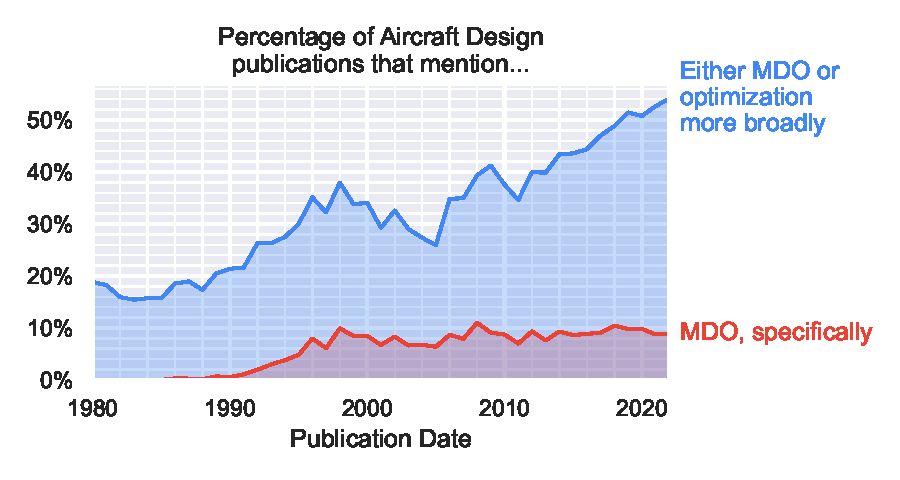
\includegraphics{../figures/mdo_citation_counts}
    \caption{Prevalance of optimization-related keywords in academic literature with the keyword ``aircraft design''. Data from Google Scholar; includes industry-standard texts such as AIAA journals and conference proceedings. MDO-specific keywords (red line) include any of: ``multidisciplinary design optimization'', ``MDO'', and ``MDAO''. The blue line adds the keyword ``optimization'' to this list.}
    \label{fig:mdo_citation_counts}
\end{figure}

This statistic alone understates the true magnitude of MDO's impact. Arguably the most pivotal contribution of MDO research to aircraft design has been to catalyze a shift towards an \textit{optimization mindset}: the recognition that optimization is not only a useful tool, but also a principled mathematical framework that can collectively represent both a design space and the engineer's design intent. Figure \ref{fig:mdo_citation_counts} shows that this mindset is a relatively recent development -- the fraction of aircraft design publications mentioning optimization in any form has tripled since the advent of MDO, reaching over 50\% today.

These optimization-based design processes have shown several benefits when used to augment traditional design methods such as point analyses, parametric surveys, and carpet plots \cite{torenbeek_advanced_2013, walton_cd_2020}. Most obviously, formal optimization methods can lead to improved design results and allow the consideration of many more design variables. Optimization can also help human designers discover clever cross-discipline synergies that might otherwise be overlooked \cite{drela_pros_1998}, and its rigor can reduce\footnote{but not eliminate} the likelihood of biased decisions \cite{torenbeek_advanced_2013}. In cases where designer intuition is exhausted, such as with unconventional configurations, optimization provides a means to identifying useful directions for further exploration \cite{drela_pros_1998}. Torenbeek argues that an optimization-based design process can respond more quickly to unexpected changes in program requirements, whereas manual processes often require substantial redesign effort \cite{torenbeek_advanced_2013}. Finally, the optimization mindset itself has benefits, even beyond the results of an optimization study. for example, discussions about problem formulation (how to translate given requirements into a quantified optimization problem) can help a team of engineers align on design goals and expose subtle discrepancies in perceived requirements\footnote{For example, is the objective to minimize fuel burn, or to maximize range? Is operating cost a quantity that should be strictly capped (a constraint), or instead only penalized (an objective)?}.

Another important area where MDO research has made significant progress is in defining the relationship between the human designer and the optimizer. The prevailing view in the early days of aircraft design optimization was that optimization would eventually advance to the point that computational tools could yield complete, production-ready designs with minimal human oversight -- as evidenced by encouraging titles such as ``Automating the Design Process'' \cite{heldenfels_automating_1973, heldenfels_automation_1974, vanderplaats_automated_1976}. Over time, this has largely given way to a more balanced view: although the optimization solve itself may be well-served by computational means, this forms only one small part of the larger design process. Inputting the engineer's design intent into the optimizer accurately (``problem specification'') and extracting intuition from the results (``interpretation'') are challenges in their own right, and best addressed by iterative human-computer teams. As described by Drela in a 1998 optimization study \cite{drela_pros_1998}, ``[Engineering optimization] is still an iterative cut-and-try undertaking. But compared to [traditional] techniques, the cutting-and-trying is not on the geometry, but rather on the precise formulation of the optimization problem.''

When considering this full design process (i.e., from initial requirements to product delivery), the scope of challenges becomes even broader. Indeed, industry adoption of MDO is often limited by non-computational user frictions \cite{salas_framework_1998, gpkit, martins_engineering_2021}. In the present work, we deliberately term these user frictions ``costs'', borrowing optimization nomenclature to emphasize that minimizing these frictions is an implied part of the objective function of any optimization-driven design process. Figure \ref{fig:birds_eye_view} summarizes a variety of design literature to present a holistic view of this complete process as applied to aircraft design \cite{torenbeek_advanced_2013, martins_engineering_2021, yang_observations_2009, torenbeek_synthesis_1976, roskam_airplane_1989, nicolai_fundamentals_2010, salas_framework_1998}. Frictions that a designer may experience from a computational optimization framework at each step are shown in \textcolor[HTML]{BB5045}{red}.

\begin{figure}[H]
    \centering
    \ifdraft{}{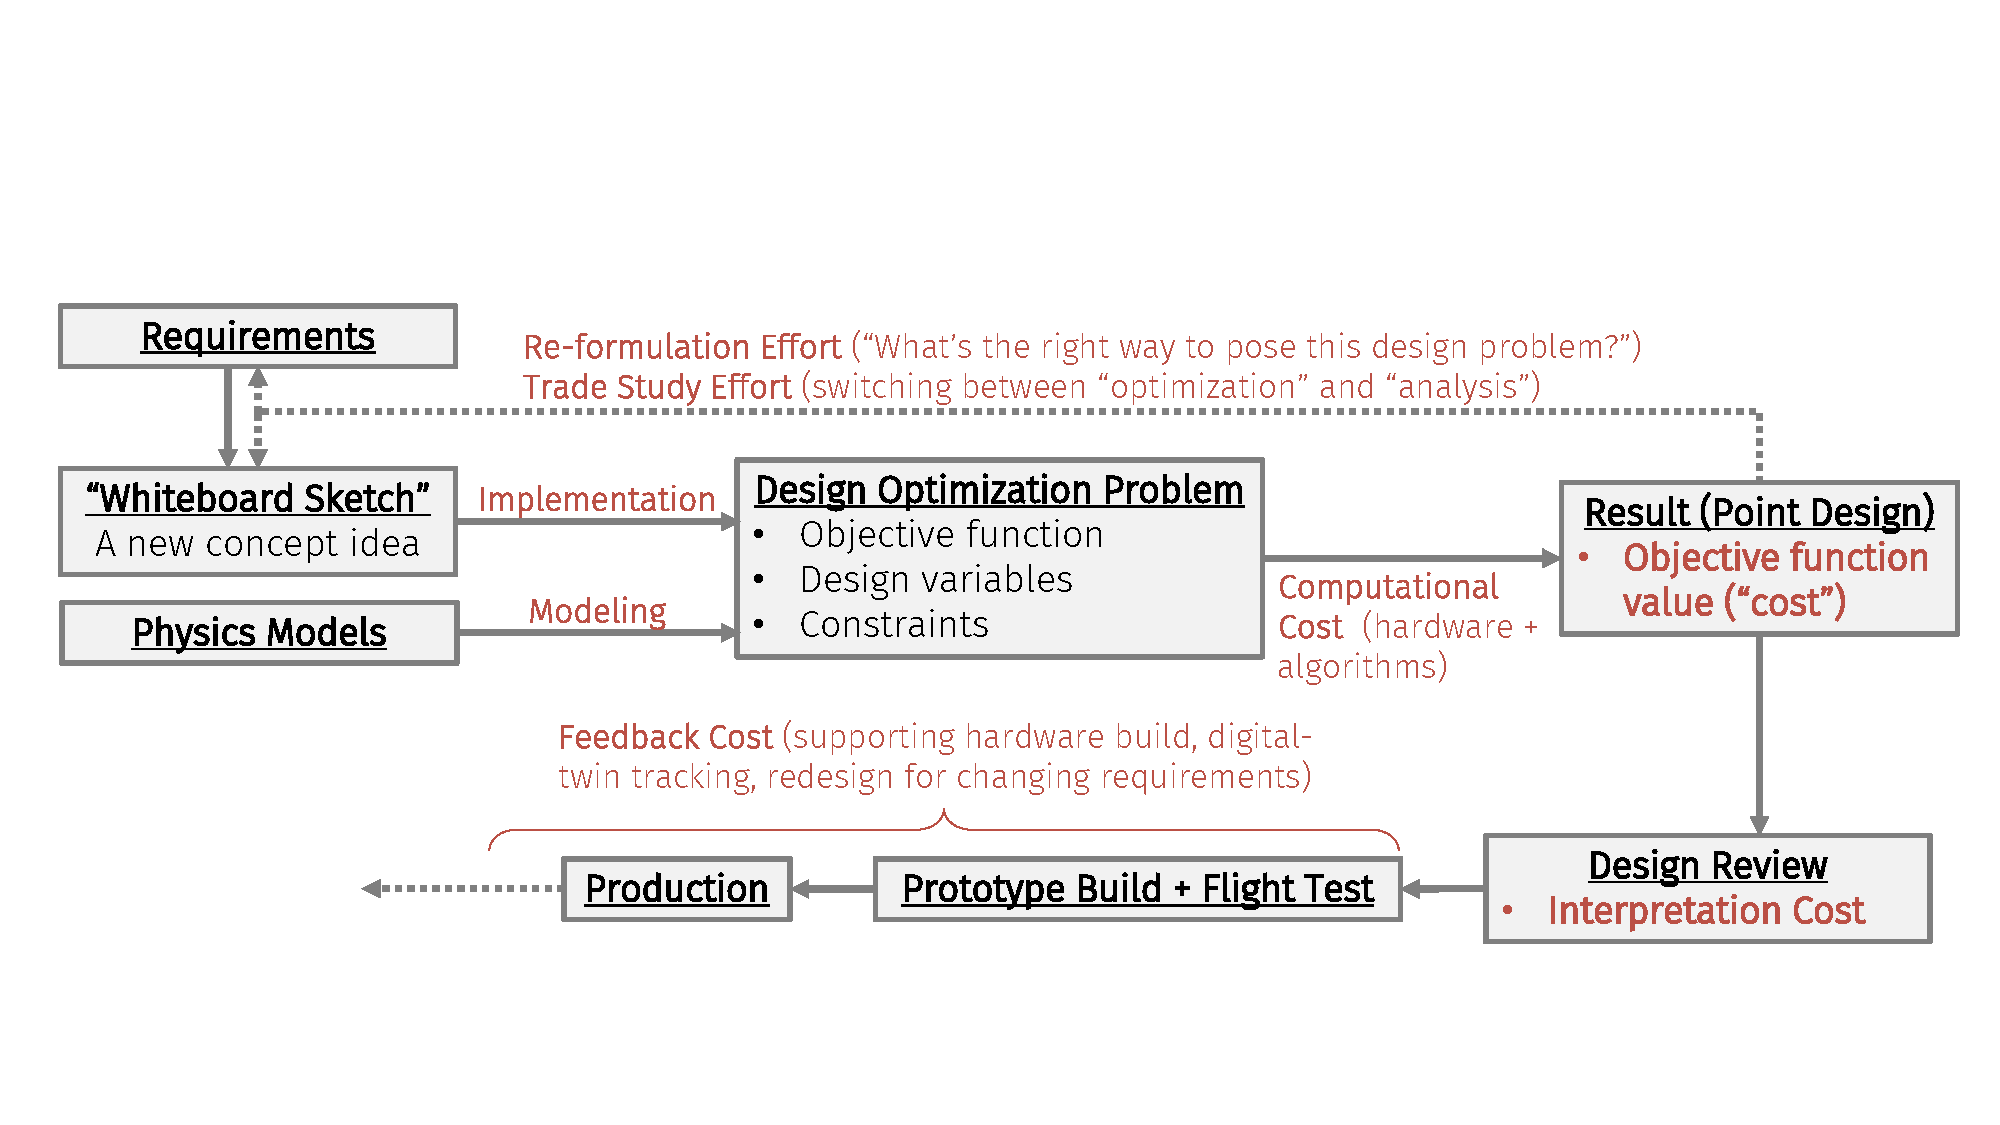
\includegraphics[width=\textwidth]{../figures/design_optimization_process_birds_eye_view}}
    \caption{A high-level overview of the optimization-driven design process, as applied to aircraft design. ``Costs'' (user frictions to be minimized) associated with each step are shown in \textcolor[HTML]{BB5045}{red}.}
    \label{fig:birds_eye_view}
\end{figure}

In the aircraft design process model of Figure \ref{fig:birds_eye_view}, the initial point of departure is a set of high-level requirements \cite{torenbeek_synthesis_1976, torenbeek_advanced_2013}. The first design step is to develop a set of candidate concepts (``whiteboard sketches''), a qualitative and configuration-focused process that largely leverages designer creativity and experience \cite{yang_observations_2009, roskam_airplane_1989}. Concepts and the associated requirements are then translated into a formal mathematical design optimization problem consisting of an objective function, design variables, and constraints. Physics models are invoked as needed to support this process; this modeling process incurs a cost that depends on the modeling flexibility of the chosen MDO paradigm \cite{sharpe_aerosandbox_2021}. The optimization problem is then solved, which incurs a computational cost and yields a point design.

This process of mapping potential concepts to problems and problems to optimized point designs is often iterative. Even for expert users, it is rare that a design optimization process will fully reflect design intent on the first attempt \cite{drela_pros_1998}. In addition, post-optimality studies may be used to assess performance robustness to off-design conditions. The total time required to close this re-formulation loop is a critical driver of how the human interacts with the MDO tool, as it directly rate-limits how much design exploration can be performed.

For a practical aircraft development program, however, this is only the beginning. The point design must survive external validation and design review by a team of subject-matter-experts; the cost of this process is a direct function of the tools an MDO framework supplies to aid result interpretability. Even beyond this, in prototyping, flight testing, production, and deployment, the design process still imposes framework requirements. For example, an analysis and optimization framework that supports a wide range of modeling fidelities has the potential to can smoothly transition from a conceptual design tool to a digital thread \cite{niederer_scaling_2021, singh_engineering_2018}. Likewise, a design tool can be used during the production process to support manufacturing decisions, such as whether an unexpected change in a component supplier still produces a feasible design with desired margins.

The remainder of this chapter will discuss some of the most important advances in optimization, design processes, and scientific computing in recent decades, with a focus on how these advances can reduce the costs incurred at various steps of this holistic process.

\subsection{Two Directions: ``Wide'' vs. ``Deep'' MDO}
\label{sec:wide_vs_deep}

Before proceeding further, it is important to clarify the scope of aircraft design optimization problems that are of interest in this thesis, as the definition of ``MDO'' is somewhat overloaded. More precisely, the modern field of MDO can be decomposed into two related but distinct subfields which have developed different strategies and mindsets to address different design needs \cite{piperni_development_2013}. Figure \ref{fig:mdo_overloaded_term} illustrates this distinction, showing how the term ``MDO'' can refer to separate tasks at different stages of the aircraft design process.

\begin{figure}[H]
    \centering
    \ifdraft{}{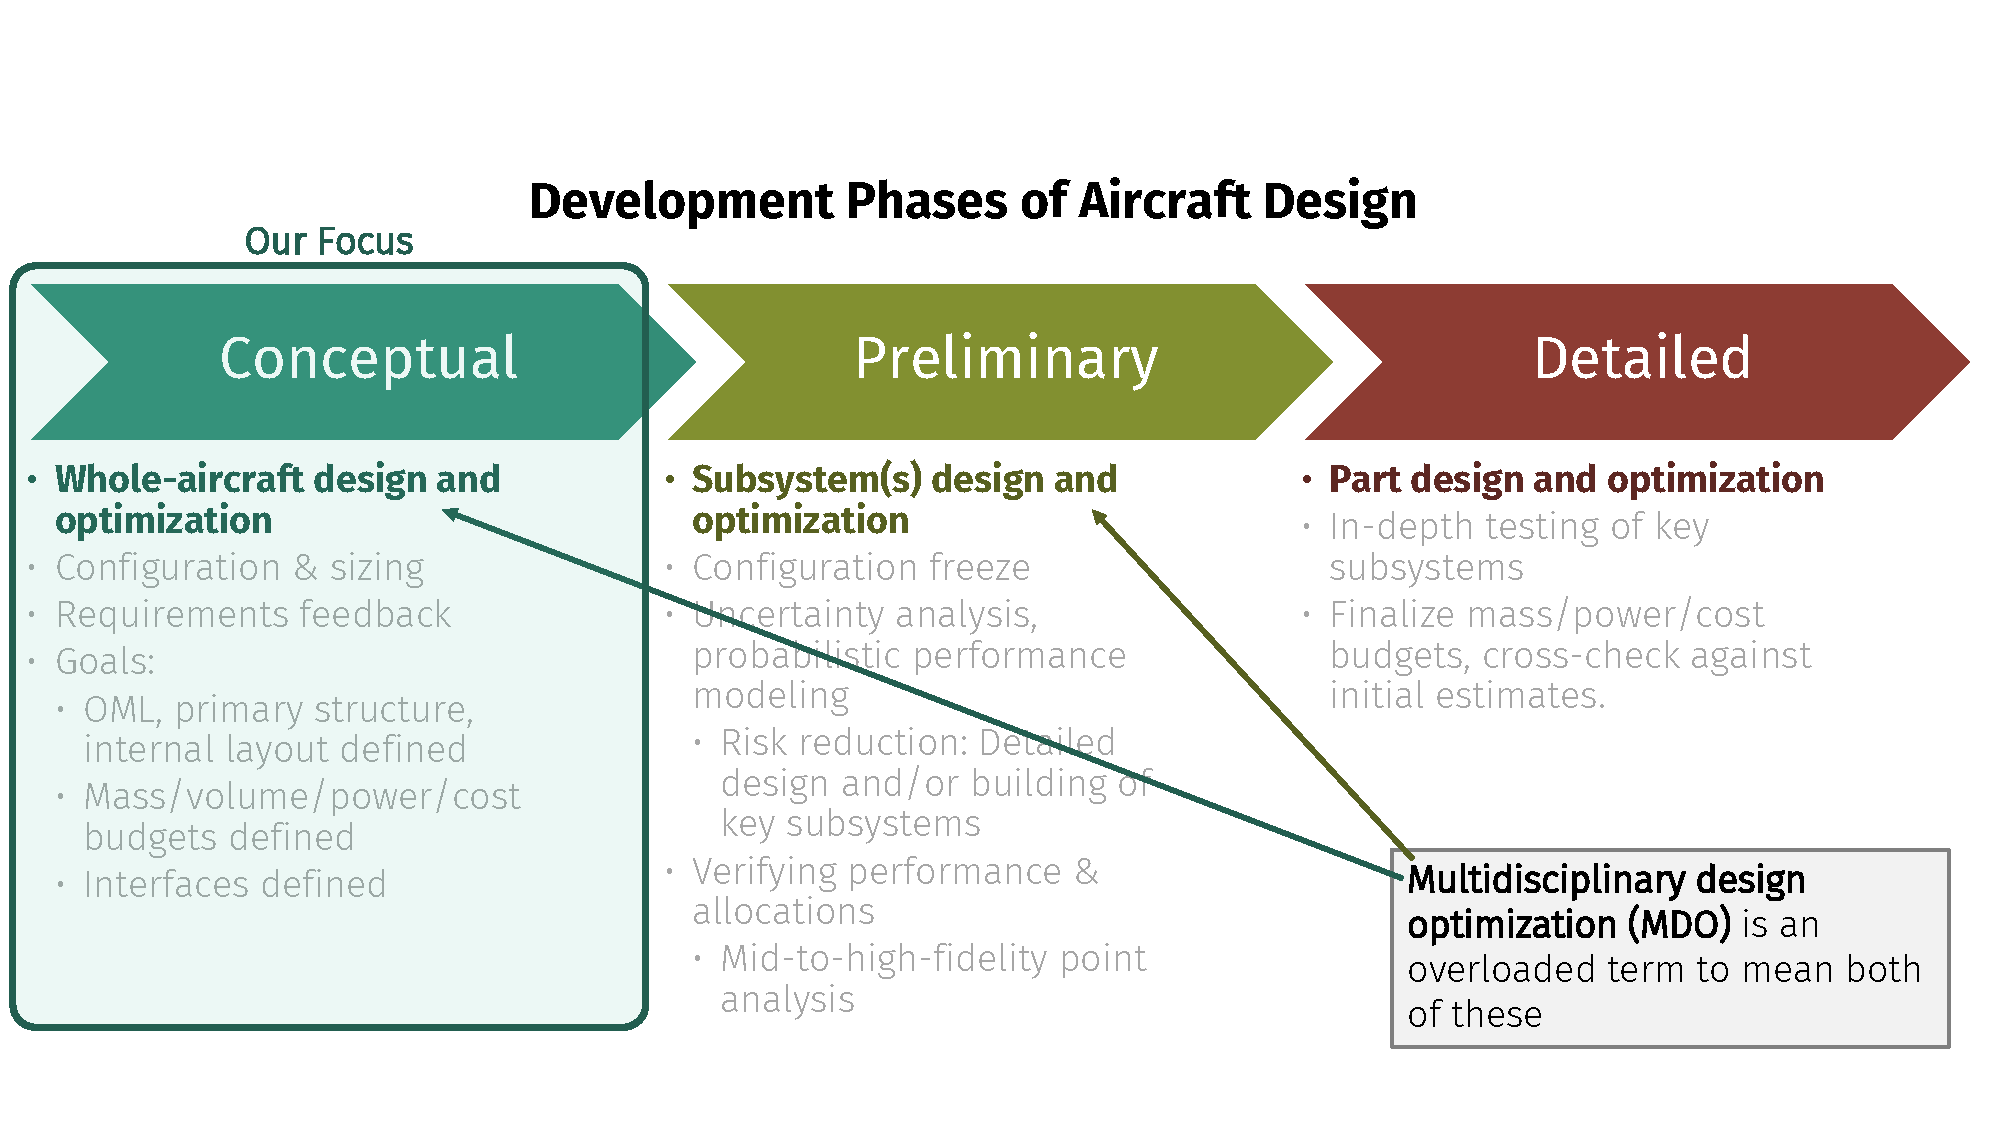
\includegraphics[trim=0cm 1.1cm 0cm 3cm, clip, width=\textwidth]{../figures/mdo_overloaded_term}}
    \caption{Multiple definitions of the term ``multidisciplinary design optimization''. Here, conceptual, or ``wide'' MDO is contrasted against preliminary, or ``deep'' MDO.}
    \label{fig:mdo_overloaded_term}
\end{figure}

The first subfield, and the subject of the present work, is that of \textbf{conceptual}, or \textbf{``wide'' MDO}. This is essentially a formalization of the conceptual sizing problem and typically involves casting a wide net to capture as many first-order dependencies as possible. The intended use case is often clean-sheet design of a complete aircraft, and the end goals are often initial identification of strong design drivers and assessment of concept feasibility. Sensitivity analysis is also a key desired output of a wide MDO process. Frameworks that tend to specialize on this class of wide MDO problems are TASOPT \cite{drela_tasopt_2010} and GPkit \cite{gpkit}.

These goals requires an enormous breadth of models to be considered, as practical aircraft designs are shaped by an enormous number of constraints that do not appear in first-principles performance analysis (e.g., the Breguet range equation). For example, a drag reduction of the vertical stabilizer is of little interest if engine-out performance constraints preclude certification; likewise, a more efficient engine is of little interest if acoustic constraints preclude customer acceptance. This need for analysis breadth can lead to design problems with many hundreds of models spanning anywhere from five to twenty relevant disciplines. To illustrate this breadth, consider the following non-exhaustive list of example disciplines that might be included:

\begin{multicols}{2}
    \begin{itemize}[noitemsep]
        \item Aerodynamics
        \item Structures and weights estimation
        \item Propulsion
        \item Power systems and thermal management
        \item Flight dynamics (trim, stability, and control)
        \item Internal geometry and packaging
        \item Mission design (concept of operations) and trajectory optimization
        \item Takeoff and landing field length analysis
        \item Certifiability, safety, and engine-out performance
        \item Life-cycle emissions
        \item Cost modeling and manufacturability
        \item Acoustic signature
        \item Ride quality
        \item Survivability and stealth
    \end{itemize}
\end{multicols}

Each of these disciplines might include dozens of submodels \cite{cruz_weight_1989, torenbeek_synthesis_1976, torenbeek_advanced_2013, drela_tasopt_2010}. To keep problems tractable despite their large scope, these models are typically low-fidelity; often, they are either derived from first principles physics with appropriate simplifications or regressions to statistical data. Despite the reduced accuracy of these models, they fulfill two critical functions. First, they apply \textit{optimization pressure} to steer the optimizer towards realistic designs, often in subtle, interdisciplinary ways. For example, increasing fuselage length requires increased landing gear length and mass to maintain a proper takeoff rotation angle, reducing the attractiveness of such design changes. Secondly, these low-fidelity models provide information on which constraints might be active near the optimum, allowing computational resources to be devoted to fidelity improvement only where it is needed. Often, these wide MDO problems are posed as large single-level optimization problems, which allows the large number of cross-disciplinary constraints to be computationally represented in a shared namespace \cite{hoburg_geometric_2014}.

The second subfield of MDO is that of \textbf{preliminary}, or \textbf{``deep'' MDO}. Here, the goal is often to provide detailed design refinement of a very close initial guess. Because the low-hanging fruit has often been picked by this stage, the design problem is often more local in nature, and the number of models is typically smaller than in wide MDO. Likewise, continued improvement from a good initial guess requires high-fidelity models, since the objective function tends to be relatively flat near the optimum and hence highly sensitive to model inaccuracy\footnote{A similar effect also occurs with constraint equations.}. For example, RANS-based CFD\footnote{Reynolds-averaged Navier-Stokes; Computational fluid dynamics} models are often used for aerodynamics, at significant cost: optimization runtimes of 1,000 to 100,000 CPU-hours are not uncommon \cite{kenway_multipoint_2014}. To maintain tractability, relatively few disciplines are considered -- often only aerodynamics and structures. The intended use case is often detailed design of a single component or subsystem, such as a wing. Due to computational challenges that tend to be more prevalent in high-fidelity models (e.g., PDE-constrained optimization, adjoint-based gradients, numerical stiffness of models, and convergence of models that use iterative solvers), the subfield of ``deep'' MDO has placed a large focus on MDO architectures that allow multi-level decomposition of the original optimization problem \cite{martins_multidisciplinary_2013}. Frameworks that tend to specialize on this deep MDO subfield are MACH-Aero \cite{he_aerodynamic_2018}, and, to some extent, OpenMDAO \cite{gray_openmdao_2019}.

While both subfields share broad similarities and provide useful design insight, they are fundamentally attacking different problems: wide MDO is aimed at clean-sheet conceptual design, while deep MDO tends to aim at detailed refinement of a close initial design. Historically, this schism became increasingly apparent roughly in the 1990s and 2000s, as various research groups began ``spending'' their increasing computational budgets in different ways: either model breadth or model depth. Examples of wide MDO research efforts in the time since this divergence include PASS \cite{antoine_framework_2005} by Kroo, TASOPT \cite{drela_tasopt_2010} by Drela, and various GPkit-based \cite{hoburg_geometric_2014} aircraft design codes. Modern ideas around deep MDO research can trace their origins to high-fidelity adjoint-based aerodynamic shape optimization studies by Alonso, Martins, and other contemporaries \cite{alonso_pymdo_2004, martins_coupledadjoint_2005, choi_multifidelity_2008}.

\subsection{Advances in Optimization Algorithms}

The current academic state-of-the-art for MDO paradigms has largely centered on two approaches: gradient-based methods with analytical gradients, and disciplined optimization methods. The former tends to be more popular in deep MDO applications, while the latter tends to be more popular in wide MDO applications; however, exceptions exist. These two existing approaches are defined and discussed in turn below. Pros and cons of these existing approaches, as compared to the proposed new paradigm, are summarized in Table \ref{tab:paradigm_comparison} of the subsequent chapter and discussed fully in Appendix \ref{chap:paradigm_comparison}.

\subsubsection{Gradient-Based Methods with Analytical Gradients}

Gradient-based optimization offer fundamental scaling advantages over gradient-free methods, and are hence preferred for large-scale design optimization when model characteristics allow \cite{lyu_benchmarking_2014, martins_engineering_2021}. The effectiveness of gradient-based methods is highly contingent on the speed and precision of gradient calculations. To illustrate this, Kirschen and Hoburg show that gradient-based optimization gives inadequate performance on even modest engineering design problems if simple finite-differencing is used \cite{kirschen}. Likewise, Adler et al. show that the inaccuracy of finite-differenced gradients can prevent accurate optimization \cite{adler_cfd_2022}.

Because of these considerations, a leading academic approach to gradient-based MDO involves manually supplying exact analytical gradients to the optimizer for each submodel. Frameworks like OpenMDAO and MACH-Aero \cite{gray_openmdao_2019} provide example implementations of this bring-your-own-gradients approach, forming the basis for several interesting case studies \cite{yildirim_performance_2021, brelje_multidisciplinary_2021, openaerostruct, bons_highfidelity_2020}. Although this paradigm is most often applied to deep MDO problems (e.g., high-fidelity aerodynamic shape optimization), it has been applied to wide MDO problems in examples such as OpenConcept \cite{brelje_multidisciplinary_2021} and OpenAeroStruct \cite{openaerostruct}.

\subsubsection{Disciplined Optimization Methods}

Another MDO paradigm that has become popular in recent years is tht of disciplined optimization methods, borrowing nomenclature from Grant \cite{grant_disciplined_2006}, Agrawal \cite{agrawal_disciplined_2019}, and Boyd \cite{boyd_tutorial_2007, boyd_convex_2004}. These methods are considered \textit{disciplined} as they impose a strict set of rules on the optimization problem formulation, which allows the optimizer to make assumptions about the problem structure (such as convexity, or log-convexity). These assumptions allow the optimizer to make more efficient use of computational resources and provide guarantees of global optimality. Geometric programming in particular has proven to be a useful disciplined MDO paradigm for aircraft design applications, as originally observed by Hoburg \cite{hoburg_geometric_2014}. GPkit \cite{gpkit, hoburg_geometric_2014, kirschen}, a framework that demonstrates this geometric programming concept targeting engineering design applications, has led to successful case studies such as the Jungle Hawk Owl aircraft \cite{jho} and Hyperloop system studies \cite{gpkit}.

\subsection{Other Advances in Design Optimization Practice}
%     complexity -- motivating the idea of general-purpose \textit{MDO frameworks} to address this as opposed to problem-specific codes

% Multipoint

% UQ


% Importance of geometry - CPACS, Haimes work
A recent notable shift in aircraft design optimization perspectives has been a renewed focus on geometry representation and parameterization. For example, Haimes and Drela \cite{haimes_construction_2012} contended in 2012 that ``constructive solid geometry (CSG) is the natural foundation for [aircraft design optimization]''. This publication extended prior work by Lazzara, Haimes, and Willcox \cite{lazzara_haimes_willcox_multifidelity_geometry_2009} that introduced the concept of ``multifidelity geometry''. Together, these works advocated for accurate 3D outer mold line representations from the earliest stages of conceptual design, with degenerate representations of this central geometry used to drive individual discipline analyses. Furthermore, they recognized the fundamental limitations of general-purpose (e.g., Parasolid-based) CAD tools in aircraft design optimization: because aerospace geometries tend to use complex, lofted surfaces, the resulting CAD models can be brittle with respect to parameter changes. This observation, along with later developments such as differentiable discretization techniques \cite{esp}, led to renewed research on how aircraft geometry should be parameterized for optimization. For example, in recent years aircraft-specific geometry tools like OpenVSP \cite{mcdonald_open_2022} and Engineering Sketch Pad \cite{esp} have been developed for design optimization workflows, a trend that arguably stems from this line of research.
% TODO transition

In a broader sense, another notable area where computational methods for aircraft design have long made inroads to industry is in inverse design tools. (An example of successful industry adoption in aerodynamics the inverse approach used by the XFoil airfoil design code \cite{drela_xfoil_1989} and others \cite{liebeck_blendedwingbody_1998} to recover a shape from a specified pressure distribution.) Like optimization methods, these inverse methods can aid designers because they offer fundamentally different capabilities than traditional design methods (e.g., carpet plots). While traditional methods focus on the ``forward problem'' (design $\rightarrow$ performance), inverse methods and optimization methods both focus on the ``inverse problem'' (performance $\rightarrow$ design). Drela \cite{drela_pros_1998} shows that this more-manual inverse approach can lead to more robust designs than optimization, if the user is not familiar with the risks of an improperly-specified optimization problem.

%    \subsection{Emerging Trends and Opportunities}
%
%
%    It would be remiss to discuss the last decade of optimization advances (and in particular, the growing recognition of the \textit{interpretability problem} of large-scale computational tools) without discussing the explosion of interest in machine learning. Learning is inherently an optimization problem to develop a generalized regressor model from given observations.
%
%    Indeed, a major criticism of generative AI in the present day is that it yields results that appear plausible on the surface level but may be deeply flawed in ways that are difficult to detect. In many ways, it is not the incorrectness, but rather the difficulty of detecting incorrectness that poses the largest threat of breaching trust. This is a problem that is not unique to AI, but rather is a fundamental challenge of large-scale computational tools in general.

\subsection{Advances in Numerical Methods}

In the past two decades several notable scientific computing techniques have matured to the point of practical use in engineering design optimization. Two of the most significant advances are automatic differentiation and automatic sparsity detection, which are discussed in detail below. A review focusing on these two techniques is available in work from Andersson et al. \cite{casadi} and Rackauckas \cite{rackauckas_generalizing_2021}. Review of several other notable scientific computing advances, such as GPU-accelerated computing, probabilistic programming, deep learning, and uncertainty quantification, are omitted here for brevity. A wider review of state-of-the-art scientific computing techniques is available from Lavin et al. \cite{lavin_simulation_2022}

\subsubsection{Automatic Differentiation}

Here, we review literature on \textit{automatic differentiation}, an advanced technique borne out of the machine learning community that fundamentally accelerates gradient-based optimization algorithms. A comprehensive modern survey is available by Baydin et al. \cite{baydin_automatic_2018}. A 2008 textbook by Griewank and Walther \cite{griewank_evaluating_2008} provides a more in-depth review of the mathematical foundations of automatic differentiation.

Gradient-based optimization methods are computationally bottlenecked by the cost of computing gradients \cite{lyu_benchmarking_2014, martins_engineering_2021}. Existing state-of-the-art workflows have users manually derive and implement highly-efficient gradients for each model, but this is time-consuming and thus impractical for early-stage design. Automatic differentiation (AD) is an efficient and accurate way to automatically compute the gradients of a function \textit{as represented in code} at runtime. In many cases, the computational complexity of this technique is fundamentally better than traditional approaches like finite-differencing; Griewank provides concrete upper bounds on the worst-case time complexity \cite{griewank_automatic_1988}.

Automatic differentiation exploits the fact that any function can be broken into a series of atomic mathematical operators, which can then be represented as a computational graph. These atomic operators, sometimes referred to as ``primitives'', may consist of mathematical operations as small as a scalar addition or as large as a solution of a nonlinear PDE (e.g., continuous adjoint methods in PDE-constrained optimization). As a practical matter, this computational graph is often created by tracing program execution with an overloaded numerics library \cite{maclaurin_autograd_2015}. This graph construction process is illustrated in Figure \ref{fig:computational-graph}. The chain rule can then be applied to this graph to compute the Jacobian of the function. Various modes of automatic differentiation effectively allow this Jacobian construction to occur either column-by-column (forward-mode) or row-by-row (reverse-mode) \cite{casadi, jax, martins_engineering_2021}; depending on the shape of this Jacobian, one strategy may be enormously more efficient than the other.

\begin{figure}[H]
    \centering
    \centerline{\begin{tikzpicture}[
    auto,
    node distance=0.8cm
]
    \tikzstyle{var} = [
    draw = c1, fill = c1!20,
    minimum height = 1cm,
    rectangle, rounded corners, thick,
    text width = 1cm, text centered,
    ]

    \tikzstyle{num} = [
    var,
    draw=c1!15!gray, fill=c1!15!gray!20
    ]

    \tikzstyle{func} = [
    var,
    draw = c2, fill = c2!20,
    ellipse
    ]

    \tikzstyle{line} = [draw, thick, ->, shorten >=2pt, shorten <=2pt]

    \node[text centered, align=center, text width = 5cm](label) {
        A computational graph for $f(a,b) = 2ab + \sin(a)$
    };

    \node[below=of label](start) {};

    \node[var, left=of start](a) {$a$};
    \node[num, right=of a](2) {$2$};
    \node[func, below=of 2](times1) {$\times$};
    \node[var, below=of a](b) {$b$};
    \node[func, below=of times1](times2) {$\times$};
    \node[func, below=of times2](sum) {$+$};
    \node[func, left=of times2](sin) {$\sin()$};
    \node[num, right=of sum, text width = 1.5cm](f) {$f(a, b)$};

    \begin{scope} [every path/.style=line]
        \path (a) -- (times1);
        \path (2) -- (times1);
        \path (times1) -- (times2);
        \path (b) -- (times2);
        \path (times2) -- (sum);
        \path (a) edge[out=-135, in=135] (sin);
        \path (sin) -- (sum);
        \path (sum) -- (f);

    \end{scope}

\end{tikzpicture}}
    \caption{A computational graph, as would be used for automatic differentiation. Reproduced from Sharpe \cite{sharpe_aerosandbox_2021}.}
    \label{fig:computational-graph}
\end{figure}

Advances in automatic differentiation (and in particular, combining this with GPU computing) are largely responsible for the revolution of practical advances in machine learning in the past decade \cite{baydin_automatic_2018}. Rackauckas in 2021 \cite{rackauckas_generalizing_2021} states: ``[Automatic differentiation] has become the pervasive backbone behind all of the machine learning libraries. If you ask what PyTorch or Flux.jl is doing that’s special, the answer is really that it’s doing automatic differentiation over some functions.'' The position of the present work is that similar scientific computing techniques can also unlock substantial practical advances in engineering design optimization.

\subsubsection{Automatic Sparsity Detection and Jacobian Coloring}

The process of gradient computation for optimization can be further accelerated if the sparsity of the constraint Jacobian is known a priori. This is because sparsity can guarantee structural independence of multiple columns\footnote{or rows, if using reverse-mode automatic differentiation} of the Jacobian, so the respective elements of the Jacobian can be evaluated simultaneously. Sparse Jacobians arise frequently in the modeling of physical systems, especially multidisciplinary ones \cite{lambe_extensions_2012}; because of this, this represents a significant opportunity in engineering design. The process of reducing the number of Jacobian evaluations by simultaneously evaluating independent columns is known as \textit{Jacobian compression} and is illustrated in Figure \ref{fig:jacobian_coloring}. To enable compression, independent columns of the Jacobian must be grouped. This process is known as \textit{Jacobian coloring}, referencing mathematical similarities to the graph coloring problem if the Jacobian's sparsity pattern is represented as a bipartite graph \cite{gebremedhin_efficient_2009}. This coloring problem does not readily admit exact solution for Jacobian sizes of interest; however, Gebremedhin et al. provide a comprehensive review of graph coloring heuristics that work well in practice \cite{gebremedhin_what_2005}. Martins and Ning provide a more concise summary that contextualizes this process around the backdrop of design optimization \cite{martins_engineering_2021}.

\begin{figure}[H]
    \centering
    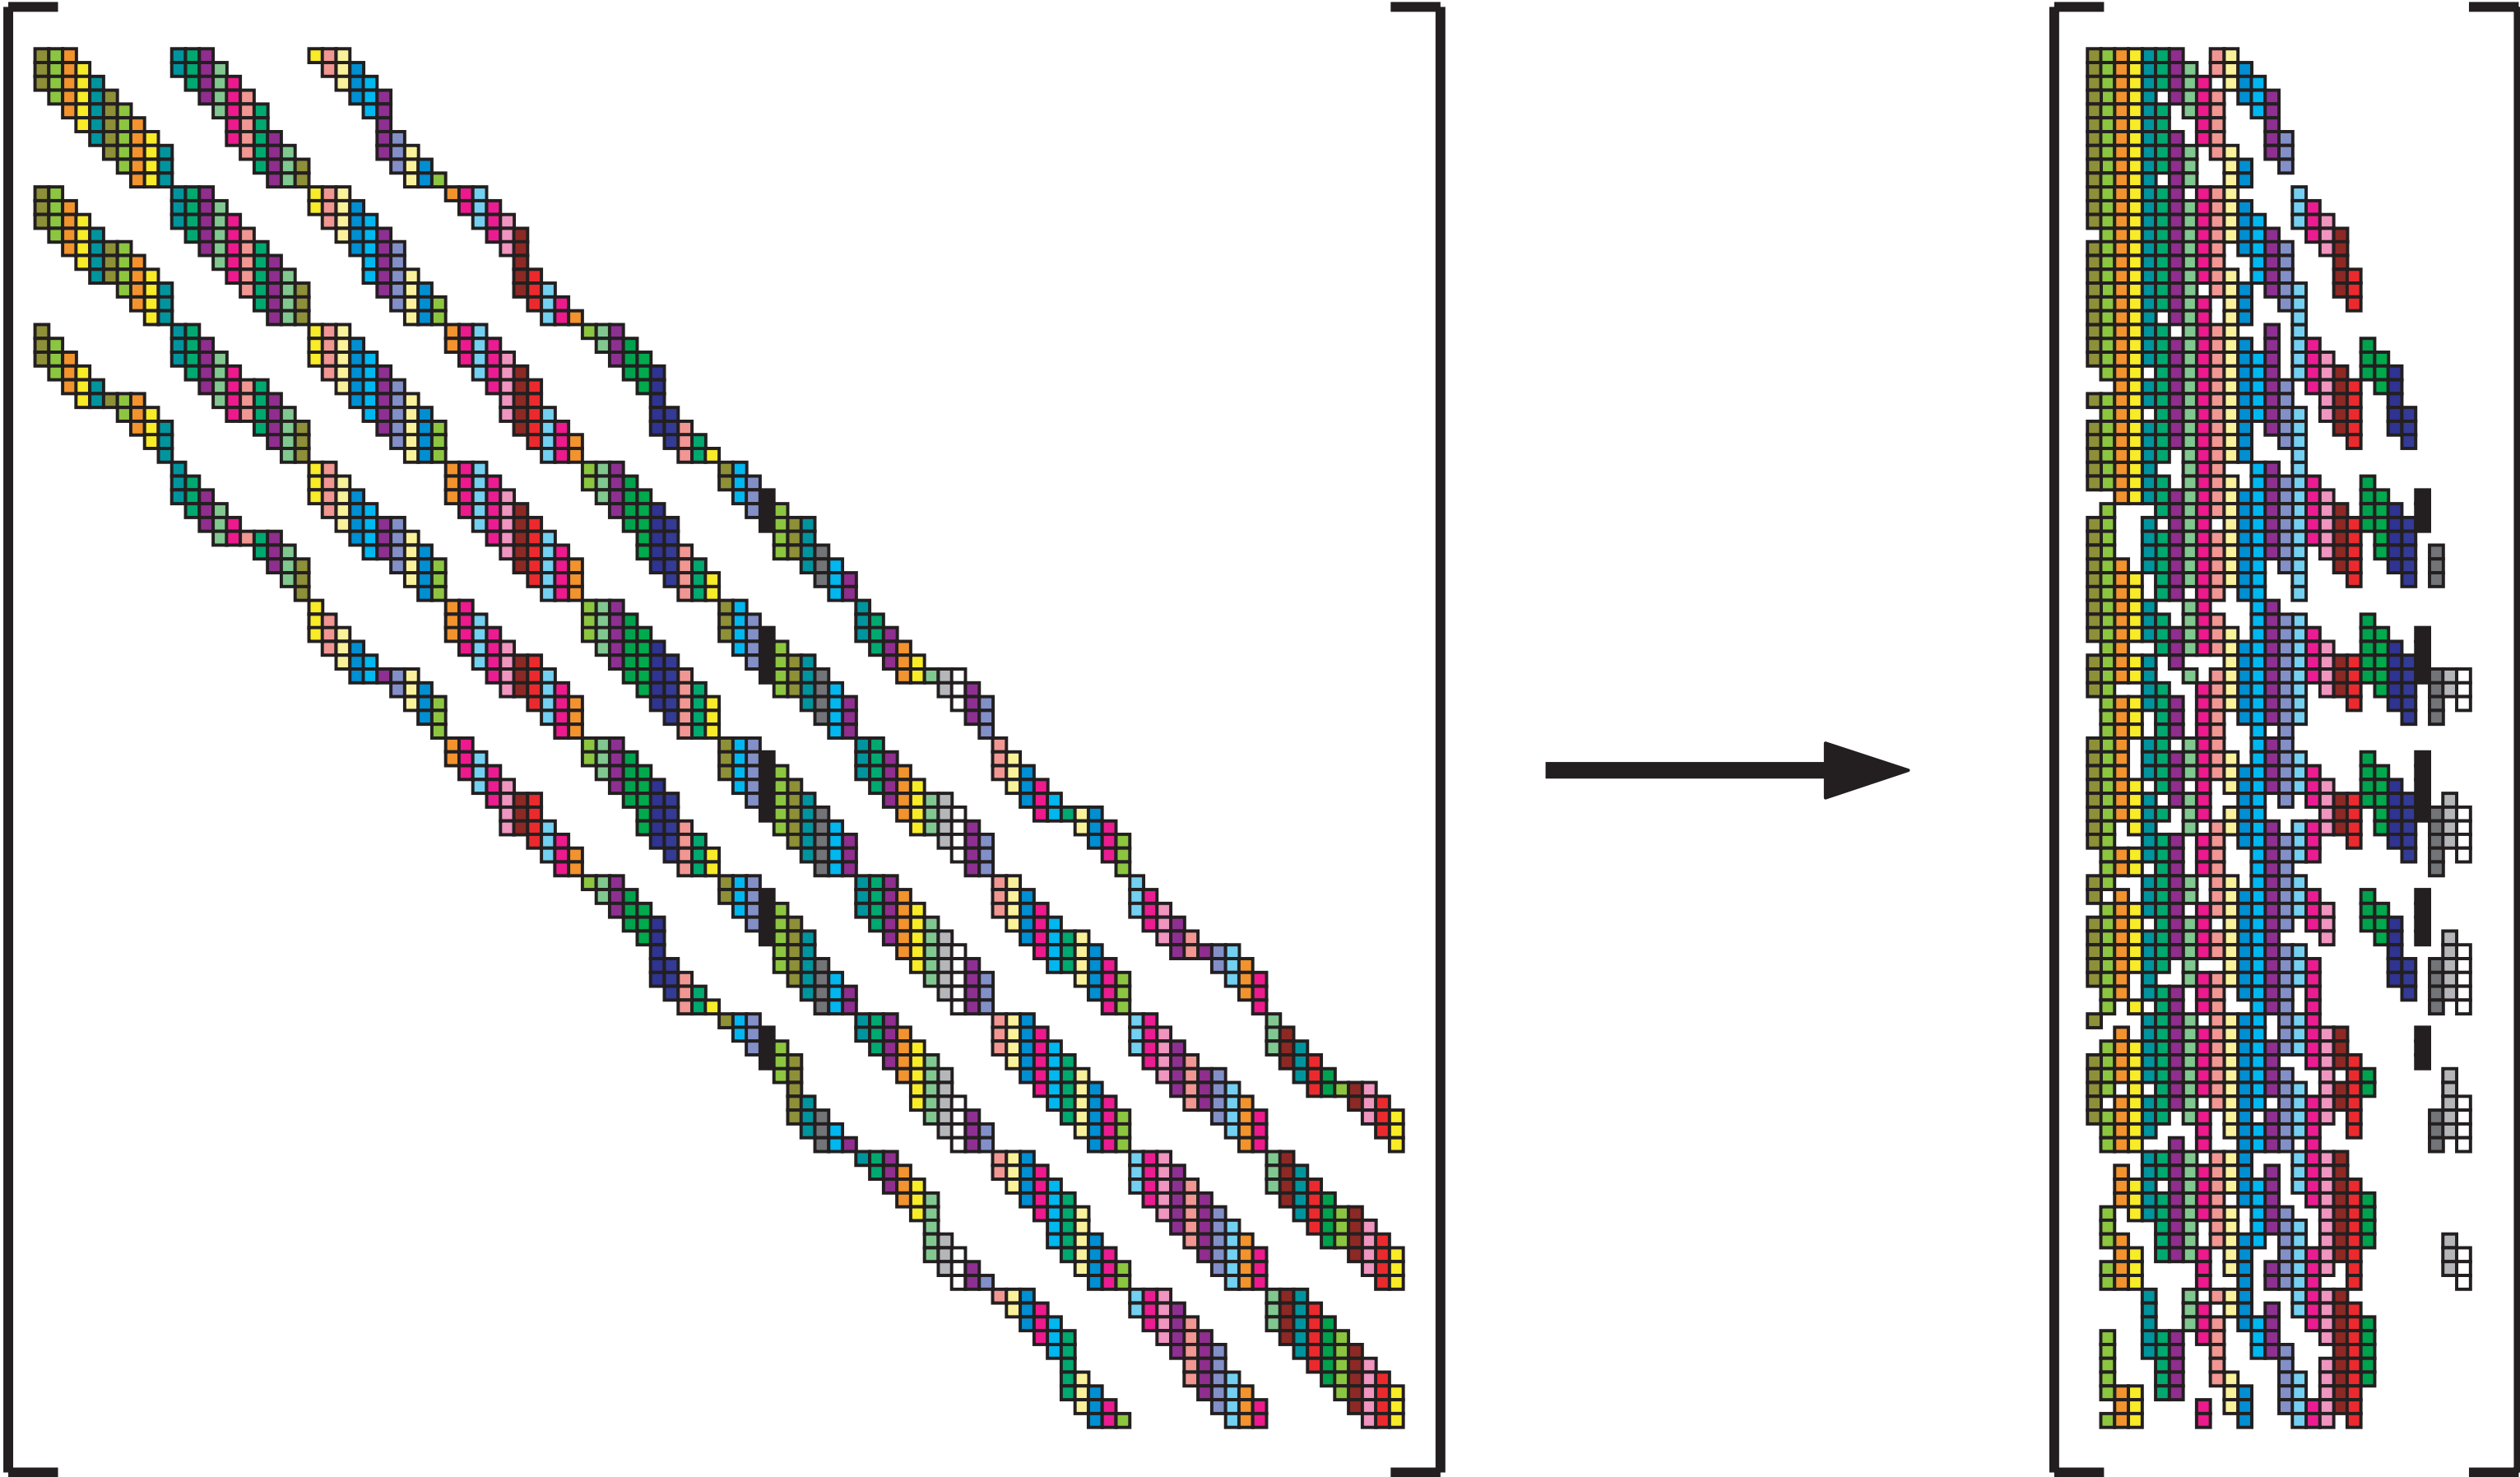
\includegraphics[width=\textwidth]{../figures/gebremedhin_2005_figure}
    \caption{A sparse Jacobian can be evaluated more quickly by simultaneously evaluating derivatives that are structurally independent, a process known as Jacobian coloring and compression. On the left of the figure is the original Jacobian; on the right is its compressed form. Figure reproduced from Gebremedhin et al. \cite{gebremedhin_what_2005}}
    \label{fig:jacobian_coloring}
\end{figure}

Before Jacobian coloring and compression can be performed, the sparsity pattern of the Jacobian must be known. This is a nontrivial task and an area of active research, with the major complications summarized by Rackauckas \cite{rackauckas_generalizing_2021}. In recent years, automated sparsity detection has enabled automatic construction of sparsity patterns using a tracing approach that is quite similar to that of automatic differentiation. This bypasses many of the potential edge-case failure modes that can occur when trying to infer sparsity purely by inspecting the dense Jacobian, such as conditional branching or cancellation. Indeed, the same computational graph can be used for this process, making this a computationally-efficient addition to a code base that already leverages automatic differentiation. Andersson et al. \cite{casadi} provide an example implementation of this automated sparsity detection within the CasADi framework. Gowda et al. provide a more complete review on state-of-the-art methods in automated sparsity detection \cite{gowda_sparsity_2019}, with state-of-the-art implementations of this by Ma et al. \cite{ma_modelingtoolkit_2021}.

%\afterpage{\FloatBarrier}


\section{Motivations for Improving Accessibility of Computational Design Optimization}
\label{sec:motivation}

This thesis focuses on improving the accessibility of advanced optimization methods for industry practitioners, with a particular focus on techniques applicable to conceptual (``wide'') MDO for aircraft. This focus is motivated by several factors.

\subsubsection*{Motivation 1: A Majority of Performance, Risk, and Cost is Committed Early}

First, the vast majority of the performance of the final design is determined by early-stage conceptual design decisions. This can manifest in both a positive and a negative sense: after the conceptual design is frozen, most design opportunities cannot be captured later and most design regrets cannot be fixed. Figures \ref{fig:motivation_1a} and \ref{fig:motivation_1b} illustrates the two sides to this coin with practical examples.

The first example, shown in Figure \ref{fig:motivation_1a}, reproduces conceptual design work on the D8 ``Double Bubble'' transport aircraft configuration by Drela \cite{drela_development_2011, drela_simultaneous_2010}. Among other technology improvements, the configuration leverages a strategy of improving passenger loading/unloading speed, which allows for a reduced cruise Mach number while retaining comparable door-to-door travel times (a surrogate for passenger acceptance). This synergistic strategy creates a feedback loop which dramatically reduces fuel burn compared to designs that are optimized on a per-component decomposition basis. For example, one of Drela's main observations from a 2010 work \cite{drela_simultaneous_2010} is that ``multi-discipline optimization considerably increases the fuel savings compared to single-discipline optimization.''

\begin{figure}[H]
    \centering
    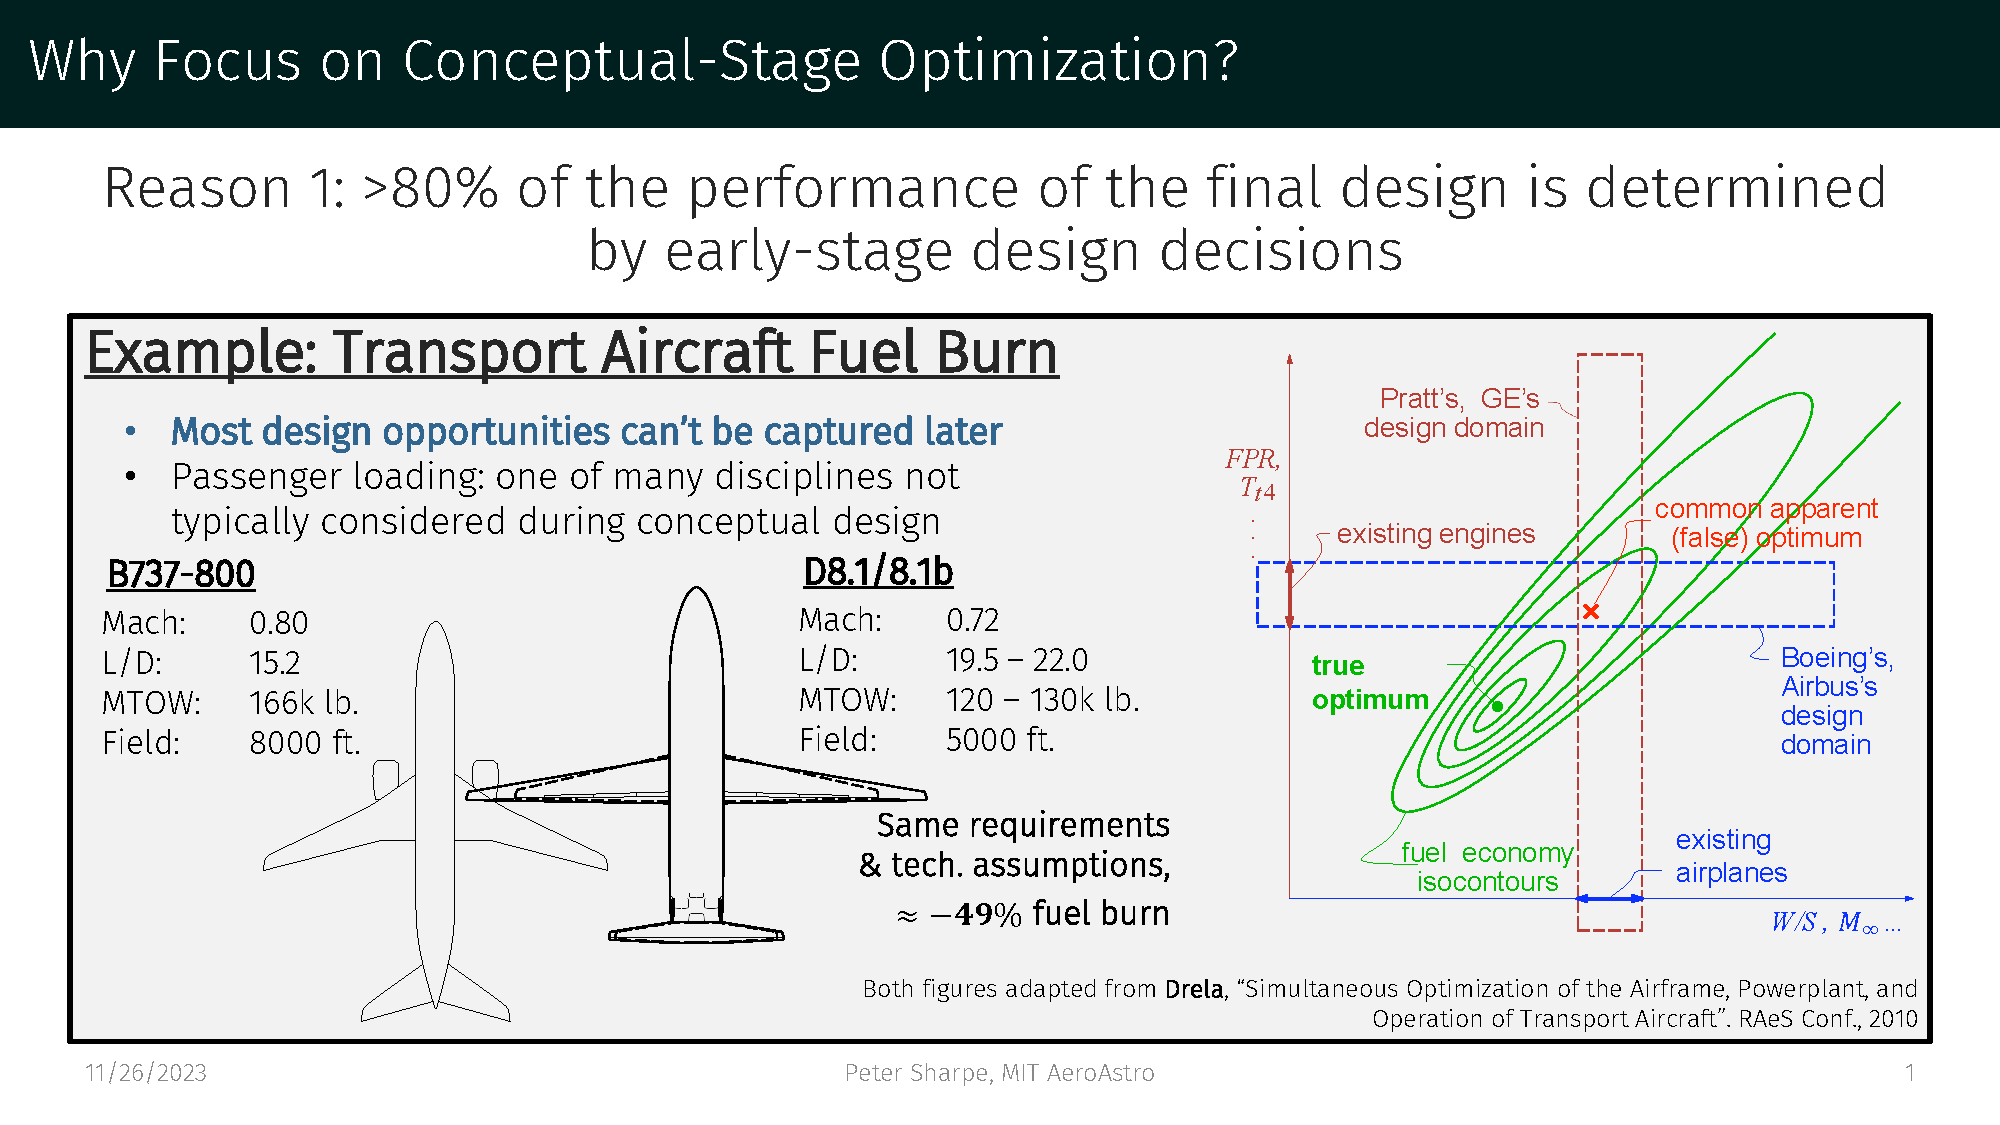
\includegraphics[page=1,trim=1cm 1.3cm 1cm 5cm, clip, width=\textwidth]{../figures/motivation_for_conceptual_MDO_focus.pdf}
    \caption{In an example from Drela \cite{drela_development_2011}, large potential fuel savings are available for transport aircraft if cross-discipline couplings are considered early in the conceptual design process. Figure elements reproduced from Drela \cite{drela_simultaneous_2010}.}
    \label{fig:motivation_1a}
\end{figure}

In a second example, shown in Figure \ref{fig:motivation_1b}, the other side of this effect is shown. Here, various electric vertical-takeoff-and-landing (eVTOL) aircraft design concepts are compared. Given the significant energy limitations of battery-powered aircraft, much of the focus of eVTOL conceptual design in the early 2010s was on traditional unit-economics performance metrics of range and payload fraction. However, as these vehicles begin to approach FAA certification and initial deployment, significant regulatory concerns have been raised about the community noise impact of such vehicles. Aeroacoustic noise, to first order, is a strong function of propulsor disk loading and blade tip speed \cite{marte_review_1970}, factors which require substantial redesign to modify later. Hence, manufacturers have had varying levels of difficulty in adapting to this renewed focus on acoustics, as this metric is largely locked in from conceptual design decisions made many years ago.

\begin{figure}[H]
    \centering
    \includegraphics[page=2,trim=1cm 1.3cm 1cm 5cm, clip, width=\textwidth]{../figures/motivation_for_conceptual_MDO_focus.pdf}
    \caption{Design regrets may arise if conceptual MDO studies do not include all relevant disciplines. This example of contemporaneous eVTOL designs assesses aeroacoustic noise, a factor that is largely determined by conceptual design decisions made many years prior. Although noise is not traditionally included in conceptual aircraft design relations, it is crucial for certification and acceptance. Thus, including many disciplines in conceptual design -- even non-traditional ones, like acoustics -- is key for avoiding major downstream design regrets.}
    \label{fig:motivation_1b}
\end{figure}

%\afterpage{\FloatBarrier}

\subsubsection*{Motivation 2: New Technologies Reignite a Need for Early-Stage Design Exploration}

A second motivation for the focus on conceptual MDO is that recent technological shifts have significantly expanded the aircraft design space compared to previous eras, calling for new tools to aid in down-selecting design concepts.

As a first example shown in Figure \ref{fig:motivation_2a}, miniaturization and uncrewed aircraft have opened up new trade spaces to explore, calling for renewed focus on first-principles early-stage design optimization. These micro-drone aircraft are able to take more risks with exotic designs, due to shorter design cycles, lower cost, and reduced certification and safety risks. New disciplines, such as packaging and folding considerations, drive new trades -- in many cases, volume allocation trades can be as sensitive as mass fraction trades in conventional aircraft. Another new trade is that of size, weight, and power (SWaP) allocations to autonomy and onboard computing. For small air vehicles, flight computer power requirements can equal or exceed propulsive power, creating new incentives that tilt the design space towards control simplicity \cite{sudhakar_balancing_2020}. New missions, particularly those that are ``dull, dirty, and dangerous'' are enabled by uncrewed aircraft with attritable design and cost optimization. Finally, physics scaling laws, like the square-cube law and transitional Reynolds numbers, cause unique concerns for small-scale aircraft that warrant first-principles conceptual design optimization.

\begin{figure}[H]
    \centering
    \begin{subfigure}[t]{0.22\textwidth}
        \centering
        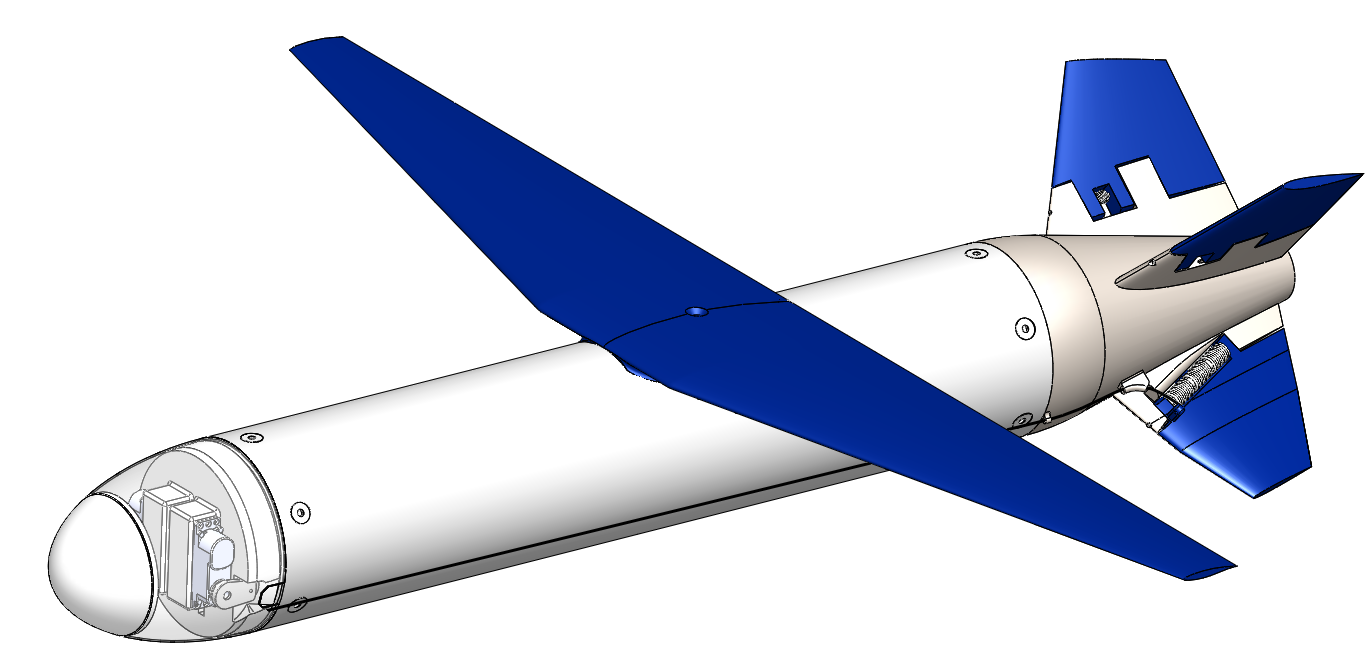
\includegraphics[width=\textwidth]{../figures/drones/firefly.png}
        \caption{MIT Firefly, a Mach 0.8, rocket-propelled micro-UAV \cite{popmech_firefly, mathesius_firefly_2019}}
        \label{fig:firefly}
    \end{subfigure}
    \hfill
    \begin{subfigure}[t]{0.22\textwidth}
        \centering
        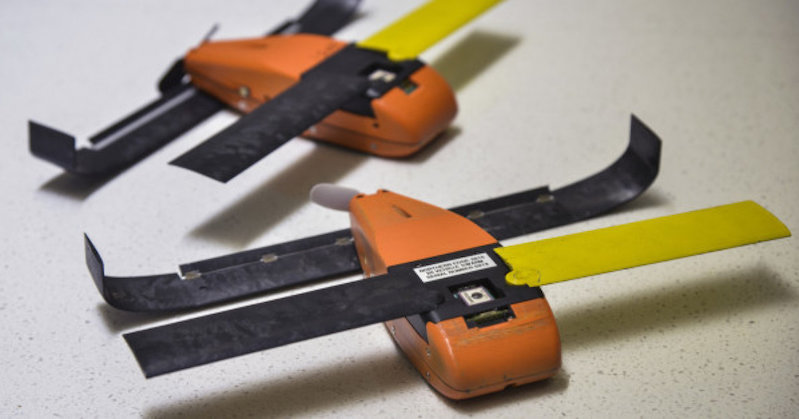
\includegraphics[width=\textwidth]{../figures/drones/perdix.jpeg}
        \caption{MIT Perdix, an air-launched ALE-55-class ISR UAV \cite{tao_design_2012}}
        \label{fig:perdix}
    \end{subfigure}
    \hfill
    \begin{subfigure}[t]{0.22\textwidth}
        \centering

        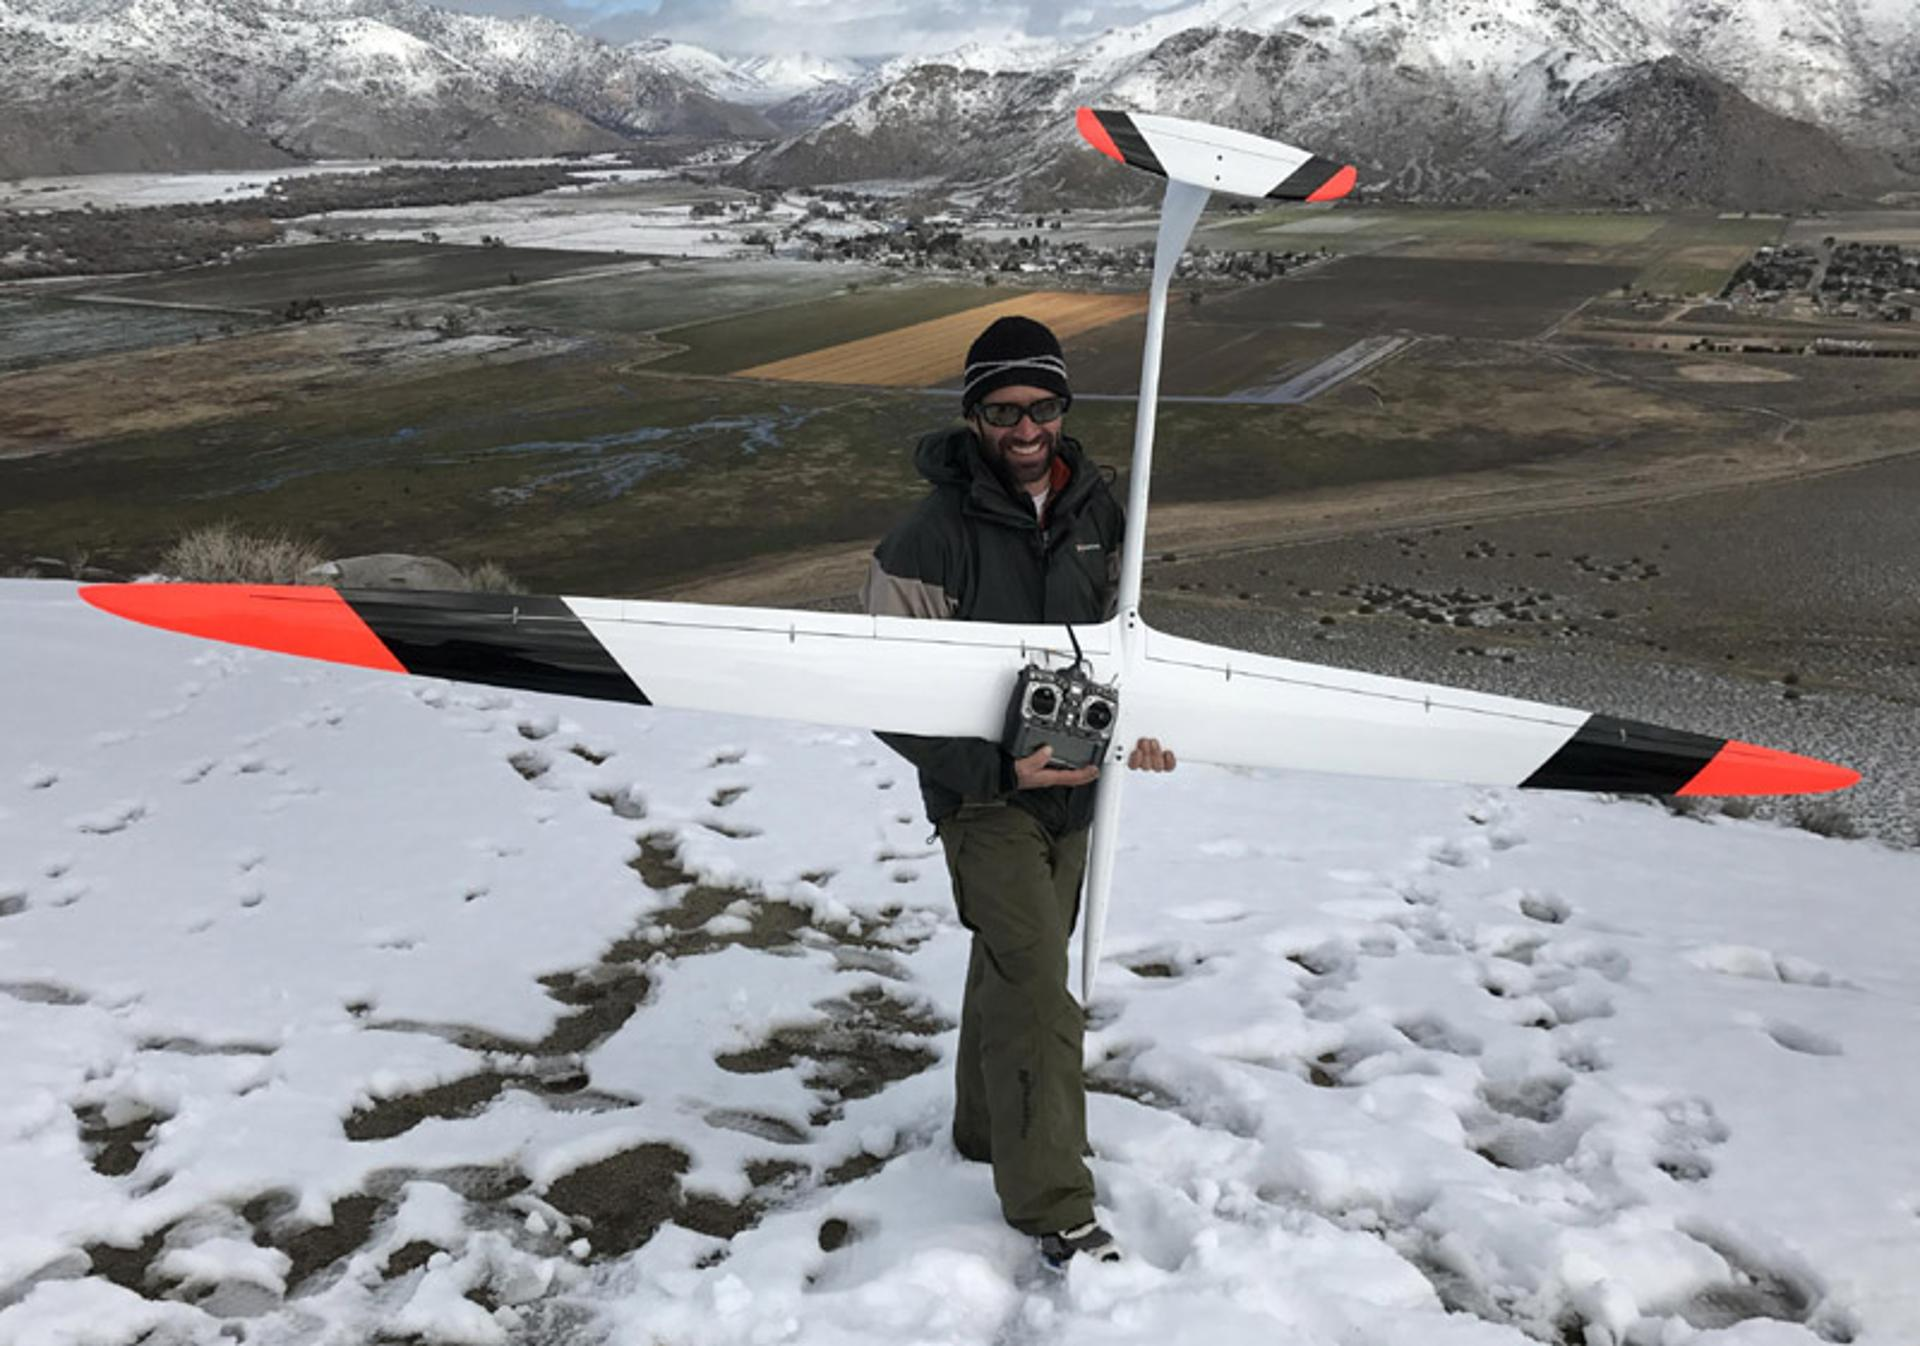
\includegraphics[width=\textwidth]{../figures/drones/transonic_dp.jpeg}
        \caption{Transonic DP, a 545-mph dynamic soaring glider with 100 G turn capability (photo: Spencer Lisenby)}
        \label{fig:transonic_dp}

    \end{subfigure}
    \hfill
    \begin{subfigure}[t]{0.22\textwidth}
        \centering
        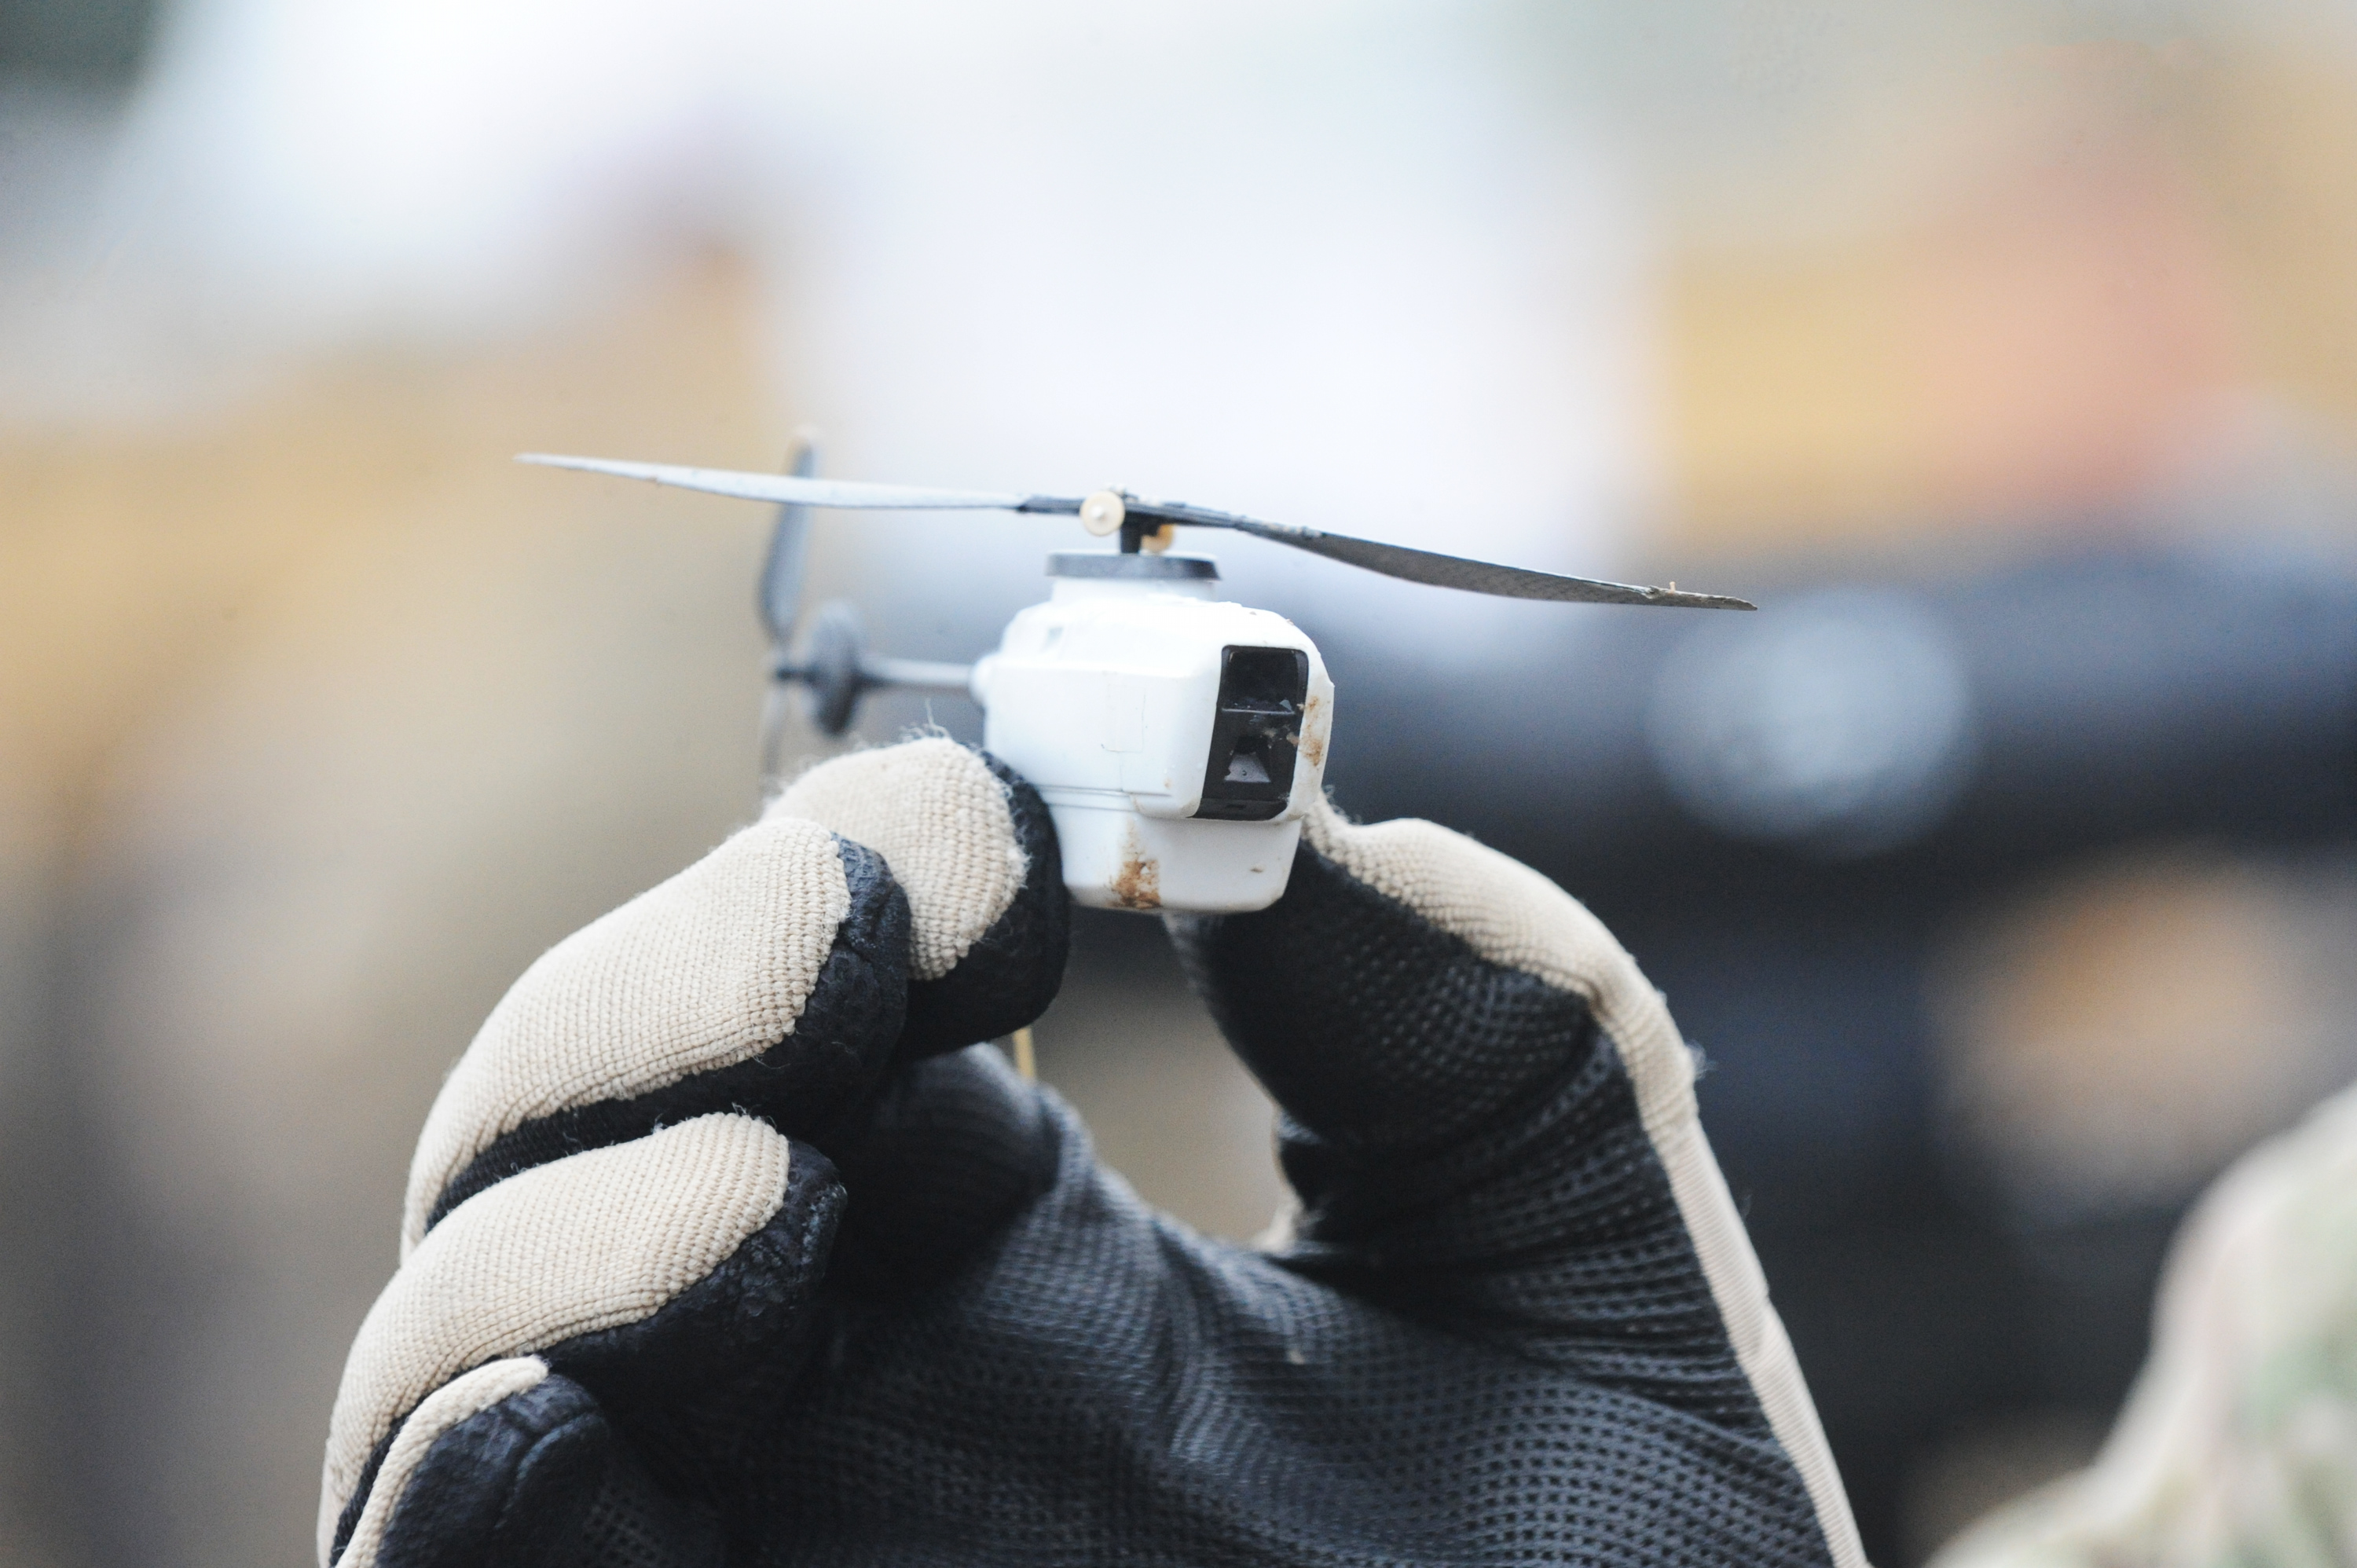
\includegraphics[width=\textwidth]{../figures/drones/hornet.jpeg}
        \caption{Black Hornet Nano, an 18-gram ISR helicopter (photo: Richard Watt/MOD)}
        \label{fig:hornet}
    \end{subfigure}
    \caption{Examples of new design spaces enabled by miniaturization and uncrewed aircraft technology in recent years.}

    \label{fig:motivation_2a}
\end{figure}

Another prominent new design space that motivates revisiting first-principles conceptual aircraft design is electric aviation, as shown in Figure \ref{fig:motivation_2b}. Electric propulsion offers a fundamentally different configuration trade space compared to conventional propulsion. In terms of energy storage, modern lithium batteries have realizable\footnote{in other words, after accounting for the generally-higher powertrain efficiencies of electric propulsion due to the lack of a thermodynamic gas cycle} specific energies that are roughly 1/25th that of kerosene, placing extreme sizing demands here. On the other hand, electric motors have excellent specific power across a wide range of size scales, dramatically fewer moving parts, and wider power bands compared to combustion engines. These factors make electric motors far more modular, essentially allowing designers to place propulsors at will -- electric aircraft with eight or more propulsors are not uncommon. The enormous design space that electric propulsion opens up is evident in Figure \ref{fig:motivation_2b}, where the diversity of aircraft configurations is wholly unprecedented compared to other aerospace domains. Part of the value proposition of conceptual MDO is that it can make rigorous design within this large space more tractable.

\begin{figure}[H]
    \centering
    \includegraphics[page=4,trim=1cm 1.3cm 1cm 5cm, clip, width=\textwidth]{../figures/motivation_for_conceptual_MDO_focus.pdf}
    \caption{Electric propulsion opens up a much larger aircraft configuration space, since electric motors offer higher specific power and modularity than combustion engines. A focus on early-stage conceptual design is critical for down-selecting from this diversity of configuration options. Figure adapted from SMG Consulting \cite{aam_reality_index}.}
    \label{fig:motivation_2b}
\end{figure}

%\afterpage{\FloatBarrier}

\subsubsection*{Motivation 3: Design Space Exploration}

The final and most significant motivation for this thesis' focus on early-stage MDO is that it provides value far beyond merely the point design that results from an optimization study. The true value of conceptual MDO is in determining which questions a design team should be asking. Examples of such questions that might be fueled by a design tool leveraging conceptual MDO are given in Figure \ref{fig:motivation_3}.

\begin{figure}[H]
    \centering
    \includegraphics[page=5,trim=0cm 3cm 0cm 6.2cm, clip, width=\textwidth]{../figures/motivation_for_conceptual_MDO_focus.pdf}
    \caption{In addition to answering specific design questions, conceptual MDO tools can help designers develop a broader intuition about the problem space and determine which questions to ask next. This figure gives examples of such exploratory questions.}
    \label{fig:motivation_3}
\end{figure}

Though some of these questions can be answered with traditional methods, like post-optimality studies and parameter sweeps, modern conceptual MDO tools can supercharge this to tens, hundreds, or thousands of design variables, allowing for a much more comprehensive exploration of the design space. The inclusion of similarly large numbers of relevant constraints effectively prunes the design space, reining unrealistic designs that a parameter sweep might otherwise yield. This capability is especially important in the early stages of a program, where the design space is often poorly understood and the design team is still developing an intuition for the problem. In this sense, conceptual MDO is a tool for \textit{design space exploration}, not just design optimization.
